\documentclass[twocolumn]{aastex631}
\received{\today}
\shorttitle{NEOCP in Era of LSST}
\graphicspath{{figures/}}

\usepackage{lipsum}
\usepackage{physics}
\usepackage{multirow}
\usepackage{xspace}
\usepackage{natbib}
\usepackage{fontawesome5}
\usepackage{xcolor}
\usepackage{wrapfig}
\usepackage[figuresright]{rotating}

% remove indents in footnotes
\usepackage[hang,flushmargin]{footmisc} 

\newcommand{\todo}[1]{{\color{red}{[TODO: #1}]}}
\newcommand{\needcite}{{\color{magenta}{(needs citation)}}}
\newcommand{\placeholder}[1]{{\color{gray} \lipsum[#1]}}

% for shorthand/consistency
\newcommand{\dig}{\texttt{digest2}}
\newcommand{\sss}{S3M}
\newcommand{\mpco}{MPCORB}

% numbers that are likely to change
\newcommand{\npernightAlg}{208}
\newcommand{\purityAlg}{5}
\newcommand{\purityAlgRaw}{10}
\newcommand{\neoLostAlg}{920}
\newcommand{\efficiencyAlg}{74}
\newcommand{\thresholdAlg}{0.7}

% custom function for adding units
\makeatletter
\newcommand{\unit}[1]{%
    \,\mathrm{#1}\checknextarg}
\newcommand{\checknextarg}{\@ifnextchar\bgroup{\gobblenextarg}{}}
\newcommand{\gobblenextarg}[1]{\,\mathrm{#1}\@ifnextchar\bgroup{\gobblenextarg}{}}
\makeatother

\begin{document}

\title{{\Large The Sky is Falling?}\\The NEOCP in the Era of LSST}

% affiliations
\newcommand{\UW}{DiRAC Institute and the Department of Astronomy, University of Washington, Seattle, WA, 98195}

\author[0000-0001-6147-5761]{T. Wagg}
\affiliation{\UW}

\author[0000-0003-1996-9252]{M. Juric}
\affiliation{\UW}

\author[0000-0003-2874-6464]{P. Yoachim}
\affiliation{\UW}

\author[0000-0002-0672-5104]{S. Cornwall}
\affiliation{\UW}

\author[0000-0001-5820-3925]{J. Moeyens}
\affiliation{\UW}

\correspondingauthor{Tom Wagg}
\email{tomjwagg@gmail.com}

\begin{abstract}
    The Legacy Survey of Space and Time (LSST) is expected to vastly increase the rate at which we observe Near-Earth Objects (NEOs). NEO candidates are presently found by specialised survey telescopes at a rate of 10-30/night, and confirmed by a network of follow-up telescopes. We present new predictions for the impact that LSST will have on the NEO confirmation page (NEOCP) -- the primary tool used for NEO candidate publication and follow-up coordination. We use mock LSST observations and the \dig{} code to predict the effect of LSST on the NEOCP when using current submission criteria. We additionally create an algorithm for predicting whether LSST will detect an object based on a single night of observations to reduce LSST's impact on the NEOCP.

    We find that, when using current submission criteria, LSST would submit between 1000 and 20,000 new objects to the NEOCP each night, 2 to 3 orders of magnitude higher than the current rates. In addition, only between 0.2 - 10\% of these objects would be NEOs, where the rest are main belt asteroids (MBAs). To reduce the necessity for external follow-up, we introduce an algorithm that predicts whether LSST itself will re-detect it, with $\efficiencyAlg{}\%$ efficiency. However, even with this algorithm enabled, LSST would still submit around $\npernightAlg{}$ objects per night on average, where only ${\sim}\purityAlg{}\%$ of them would be NEOs. We conclude that the best course of action may be {\em not} to attempt follow-up of LSST NEOs for the first 1-2 years of the survey, until most of the MBA background is catalogued.
\end{abstract}

\keywords{Near-Earth objects, Asteroids, Solar system, Small Solar System bodies, Surveys}

\section{Introduction} \label{sec:intro}
Near-Earth Objects (NEOs) are asteroids and comets that have a perihelion distance less than $1.3 \unit{AU}$. It is estimated that approximately one fifth of this population passes close enough to Earth that small perturbations in their orbit may lead to intersections with the Earth's orbit and potential collisions \citep[e.g.][]{Jones+2018}. A subset of these objects are known as Potentially Hazardous Asteroids (PHAs), these objects are defined as being at least 140m in diameter that pass within 0.05AU of the Earth\footnote{\url{https://cneos.jpl.nasa.gov/about/neo_groups.html}}. PHAs are large enough to make it through the Earth's atmosphere and still cause significant damage through impact. Given the threat posed by these objects, it is therefore critical that we catalogue and determine the orbits and sizes of NEOs.

The Minor Planet Center maintains a catalogue of known NEOs and their orbits\footnote{\url{https://www.minorplanetcenter.net/iau/MPCORB/NEA.txt}}, as well as the NEO confirmation page (NEOCP\footnote{\url{https://www.minorplanetcenter.net/iau/NEO/toconfirm_tabular.html}}), which lists newly discovered NEO candidates that should be prioritised for additional observations by the NEO follow-up community. These community follow-up observations constrain the trajectory of objects over time and are often necessary for fully constraining the orbit of an object. An object is only listed on the NEOCP when it has a high probability of being an NEO. This probability is quantified using the \dig{} code, which assigns a score between 0 and 100 and only objects with a score of 65 or more are listed on the page \citep{Keys+2019}. Currently, on average around two dozen objects are added to the NEOCP on each night.

The Legacy Survey of Space and Time \citep[LSST,][]{Ivezic+2019} will rapidly increase the rate at which NEOs are discovered and sent to the NEOCP. \citet{Jones+2018} showed that at the end of the 10-year LSST baseline survey the completeness of NEOs with an absolute magnitude of $H \le 22$ would be 73\%. Most of these objects will be discovered using ``tracklet linking'': a computational technique where at least three pairs of observations (``tracklets'') observed over a 15-night period are identified as belonging to the same object (Heinze et al., in prep). The orbits of objects discovered with this technique will typically be reasonably well known, and in need of no immediate follow-up. However, this tracklet linking comes at a cost: the object is not identified as interesting until the third tracklet is imaged -- at best, three nights after the first observation or, at worst, nearly two weeks later. This means that potentially interesting (or hazardous) objects may be missed until it's too late to observe (or react to) them.

A more traditional discovery technique would be to take enough back-to-back images so high-confidence tracklets can be built with three or more observations and immediately reported for follow-up. The LSST cannot do that, as it would reduce the efficiency of other science areas the data are to support. However, in a smaller area of the sky (e.g., where there are adjacent field overlaps), the LSST {\em does} serendipitously produce 3+ observation tracklets. Such tracklets could be immediately identified and submitted to the MPC for possible inclusion to NEOCP.

Even with just serendipitously observed 3+ observation tracklets, there is a concern that the number of objects so submitted to the NEOCP may increase by several orders of magnitude. This would present problems for the follow-up community as it would not be possible to follow up each submitted object. Particular objects would need to be prioritised but regardless many objects would still be missed and receive no follow-up. However, a large number of the objects that LSST observes will be re-observed and discovered by LSST alone, though there will still be a sizeable fraction of objects that require community follow-up. It is therefore important to identify this fraction so that the follow-up community can effectively prioritise observations.

The aim of this paper is to quantify the impact of LSST on the NEOCP and consider possible strategies to mitigate this impact. We performed mock LSST observations and used \dig{} to assess the number of objects observed by LSST would be submitted to the NEOCP. Confirming the concern that this number would be too large to act on, we look at the mitigation strategies. We present an algorithm for predicting whether LSST will later re-detect an object given a single night of observations (therefore making community follow-up unnecessary). We applied this algorithm to the mock observations and quantified by how much we could reduce the number of objects requiring community follow-up.

Our paper is structured as follows. In Section~\ref{sec:current_impact}, we estimate the impact that LSST will have on the NEOCP when applying current submission criteria. We describe the methods for simulating LSST observations, calculating \dig{} scores and present our findings for the total number and type of objects submitted to the NEOCP by LSST. In Section~\ref{sec:mitigation}, we present an algorithm for prediction of LSST self-followup probabilities and assess how well its application reduces the impact on the NEOCP. Based on these results, in Section~\ref{sec:discussion} we make recommendations for how objects should be submitted to the NEOCP from LSST. We conclude in Section~\ref{sec:conclusion}.

\section{The impact of LSST using current submission criteria}\label{sec:current_impact}
In order to make predictions for the NEOCP in the era of LSST, we make simulated observations of a catalogue of solar system objects that takes into account currently known objects. We then use the \dig{} code to calculate NEO scores for each object and use these values to make predictions for the NEOCP.

\subsection{Simulated Observations}
We start by developing a `hybrid' solar system object catalogue to investigate the effect of LSST sources on the NEOCP. This catalogue contains both real and synthetic objects, whilst retaining the same overall distributions in position, velocity and absolute magnitude found in the purely synthetic catalogue (see Appendix~\ref{app:hybrid}). This makes it possible to exclude already discovered objects from the simulated lists of objects the LSST will find.

We then use this catalogue to perform mock LSST observations using a baseline v2.1 10 year \texttt{OpSim} simulation \citep{opsim, Cornwall+2020}. These observations account for both scheduled and unscheduled downtime and simulate the current baseline observing strategy that will be followed by LSST. The resulting simulations span 3653 days, and have over 50 million observations. An example of asteroids detected in a single night of observations is shown in Figure~\ref{fig:observations_per_night}.

\begin{figure}
    \centering
    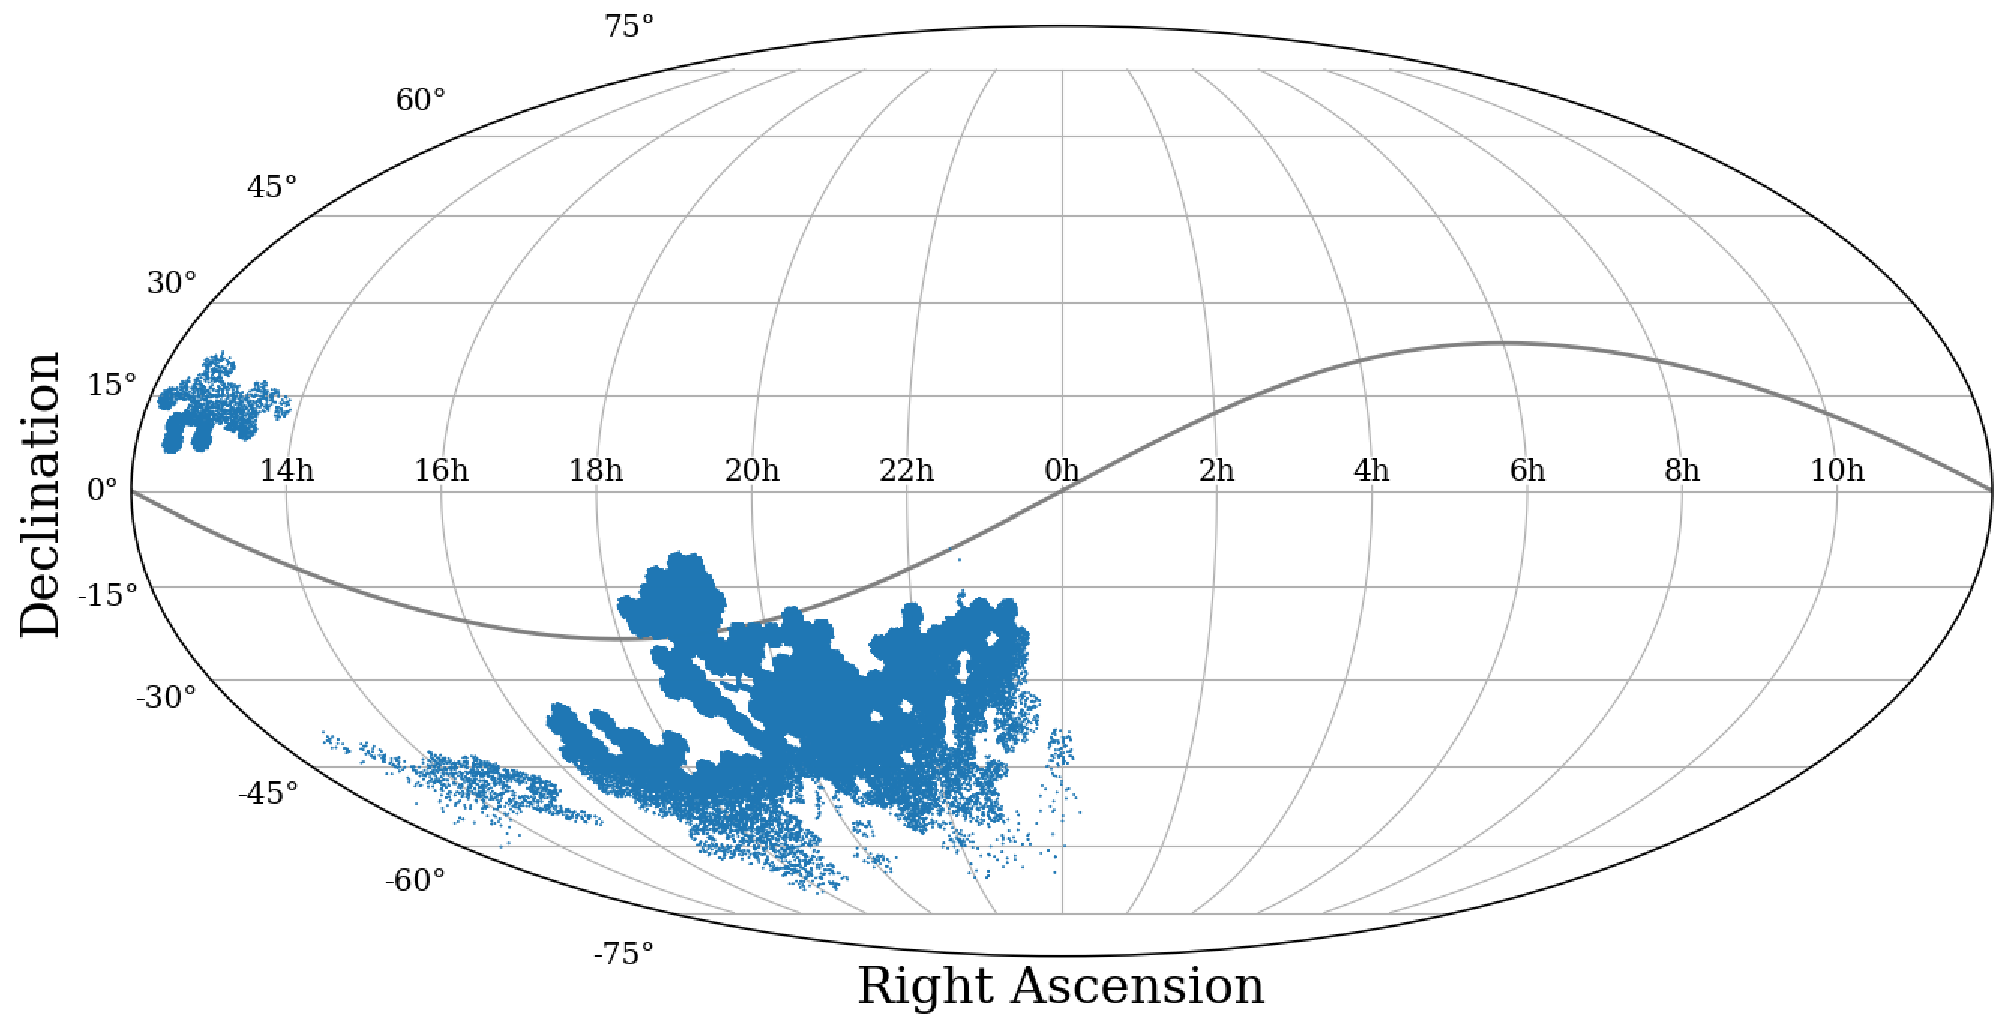
\includegraphics[width=\columnwidth]{observations_placeholder.pdf}
    \caption{An example of asteroids that are detected in a single night of LSST observations. This example shows night 130 of the simulated observations, with ${\sim}420,000$ observed asteroids, of which ${\sim}1000$ are NEOs. Grey curve indicates the ecliptic plane.}
    \label{fig:observations_per_night}
\end{figure}

\subsection{\dig{} Score Calculation}\label{sec:digest2_score}
The main criterion the Minor Planet Center uses to place an object on the NEOCP is an NEO \dig{} score of at least 65. This score, ranging from 0 to 100, assesses the probability that the object is an NEO and is calculated using the eponymous \dig{} code \citep{Keys+2019}.

\dig{} compares a simulated catalogue of solar system objects to observed tracklets to estimate the probability that an object is an NEO. \dig{} bins simulated objects into 15 different orbit classes and uses bins of perihelion, eccentricity, inclination and absolute magnitude. Then, for each observed tracklet, \dig{} samples a series of possible distances and radial velocities and uses those values to estimate possible orbits of the object. These orbits are binned in the same way and assigned a class based on this. The NEO score is then estimated as a fraction of the orbits that are classified as NEOs. For a more exhaustive description of \dig{}, see \citet{Keys+2019}.

We use \dig{} to calculate the NEO score of each NEO and MBA in the hybrid catalogue that is observed in the first year of observations. We apply three further cuts based on the Rubin observatory system specifications before considering which submissions are eligible for the NEOCP \citep{oss}.
\begin{enumerate}
    \item \textbf{Number of observations:} We consider only objects which have at least 2 observations on a given night (though we investigate the effect of making this limit more stringent - see Section.~\ref{sec:traffic_basic}).
    \item \textbf{Minimum arc length:} We ensure that each tracklet is at least 1 arcsecond in length. This ensures that the motion vector of the tracklet can be well determined.
    \item \textbf{Maximum time separation:} We set the maximum time between observations to 90 minutes. Thus we only allow tracklets that have at least one pair of observations that occur within 90 minutes of each other.
\end{enumerate}
The motivation behind these cuts is to ensure that the orbit of the object is well constrained, such that its position at a later time can be accurately determined. With few observations or short tracklets, many different orbits could reproduce the same motion on the sky. Moreover, observations that are separated too significantly in time may be spurious linkages, where observations of multiple objects are incorrectly assumed to be of the same source.

\begin{figure}[b]
    \centering
    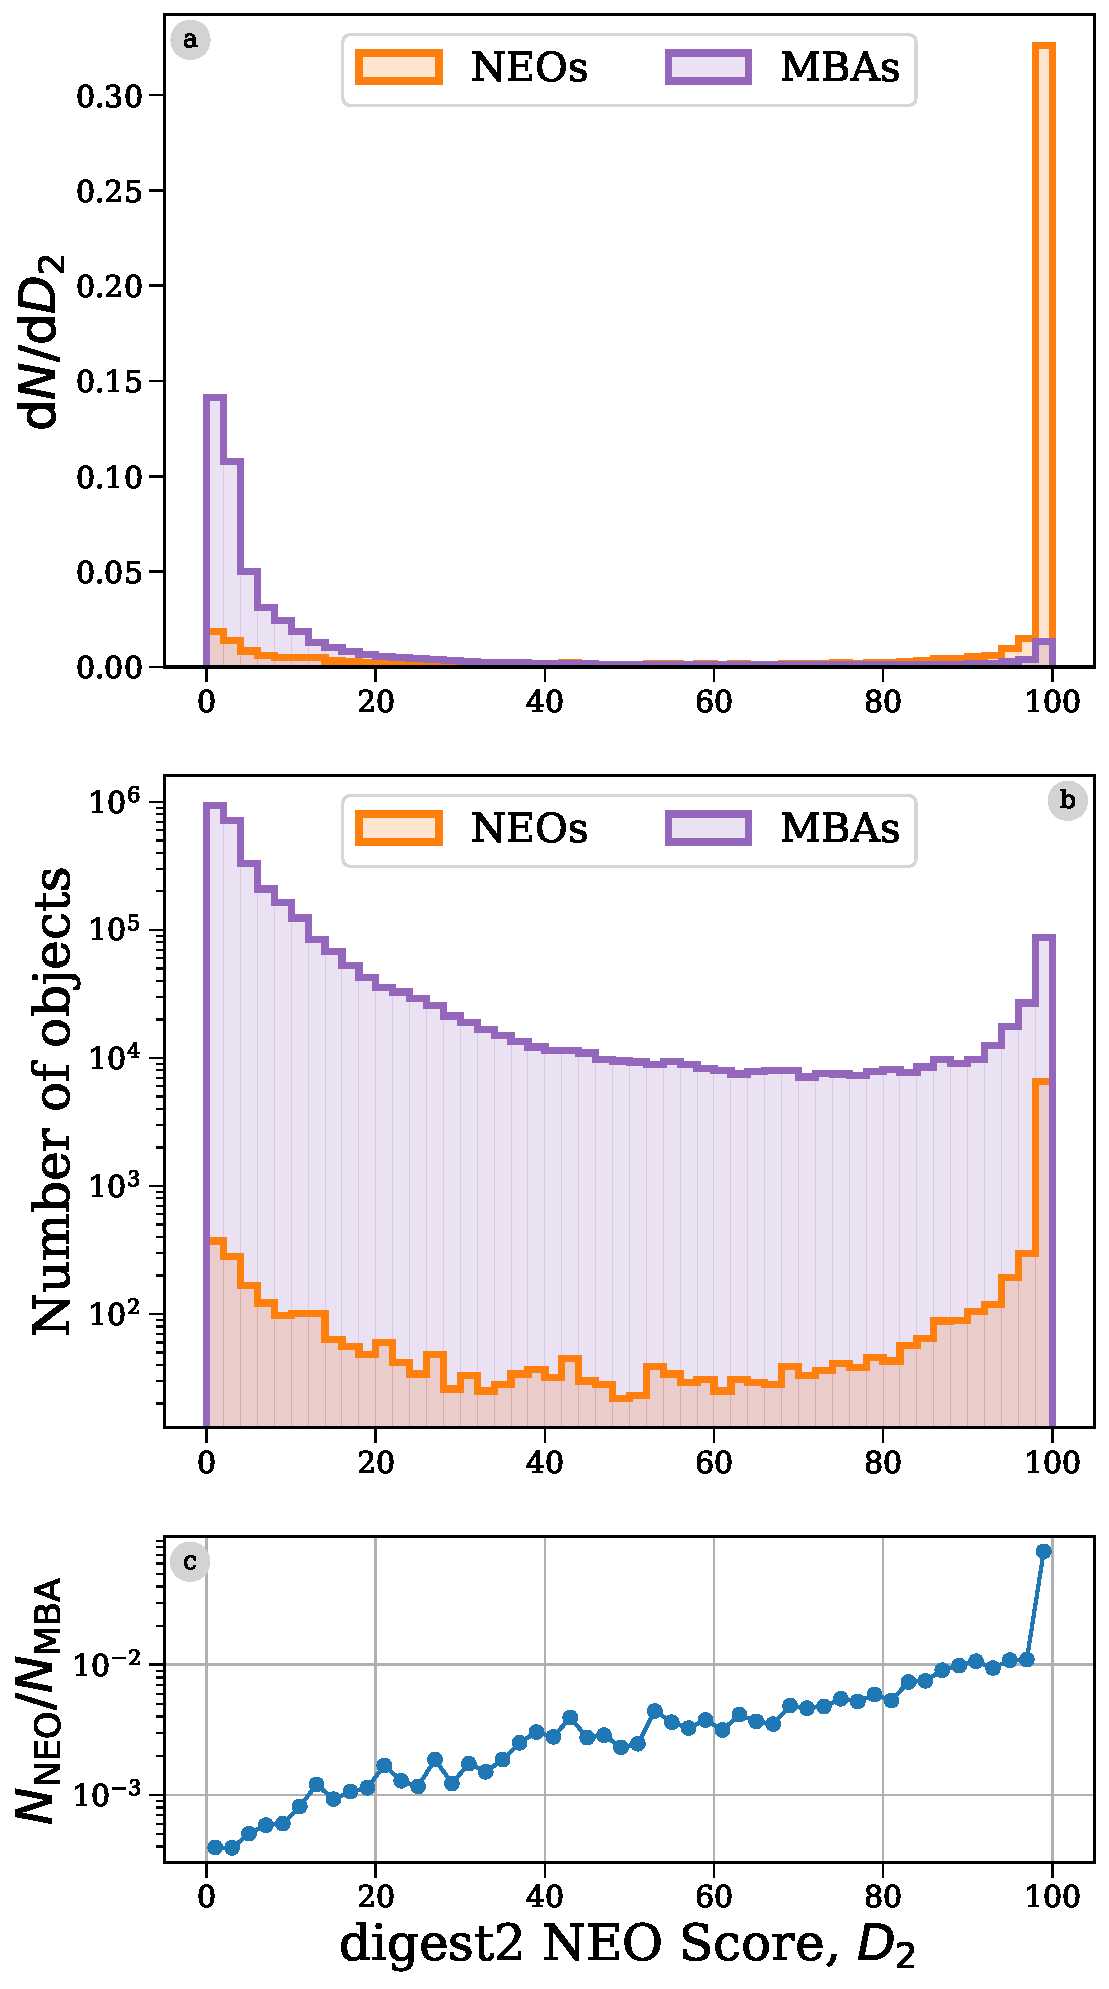
\includegraphics[width=\columnwidth]{digest2_pollution.pdf}
    \caption{\dig{} scores for all NEOs and MBAs observed in the first year of our simulated LSST observations. \textbf{(a)} normalised histograms of \dig{} scores, \textbf{(b)} the same histograms un-normalised \textbf{(c)} ratio of the histograms in (b). Note that the latter two panels are on a logarithmic scale.}
    \label{fig:digest2_example}
\end{figure}
\begin{figure*}[htb]
    \centering
    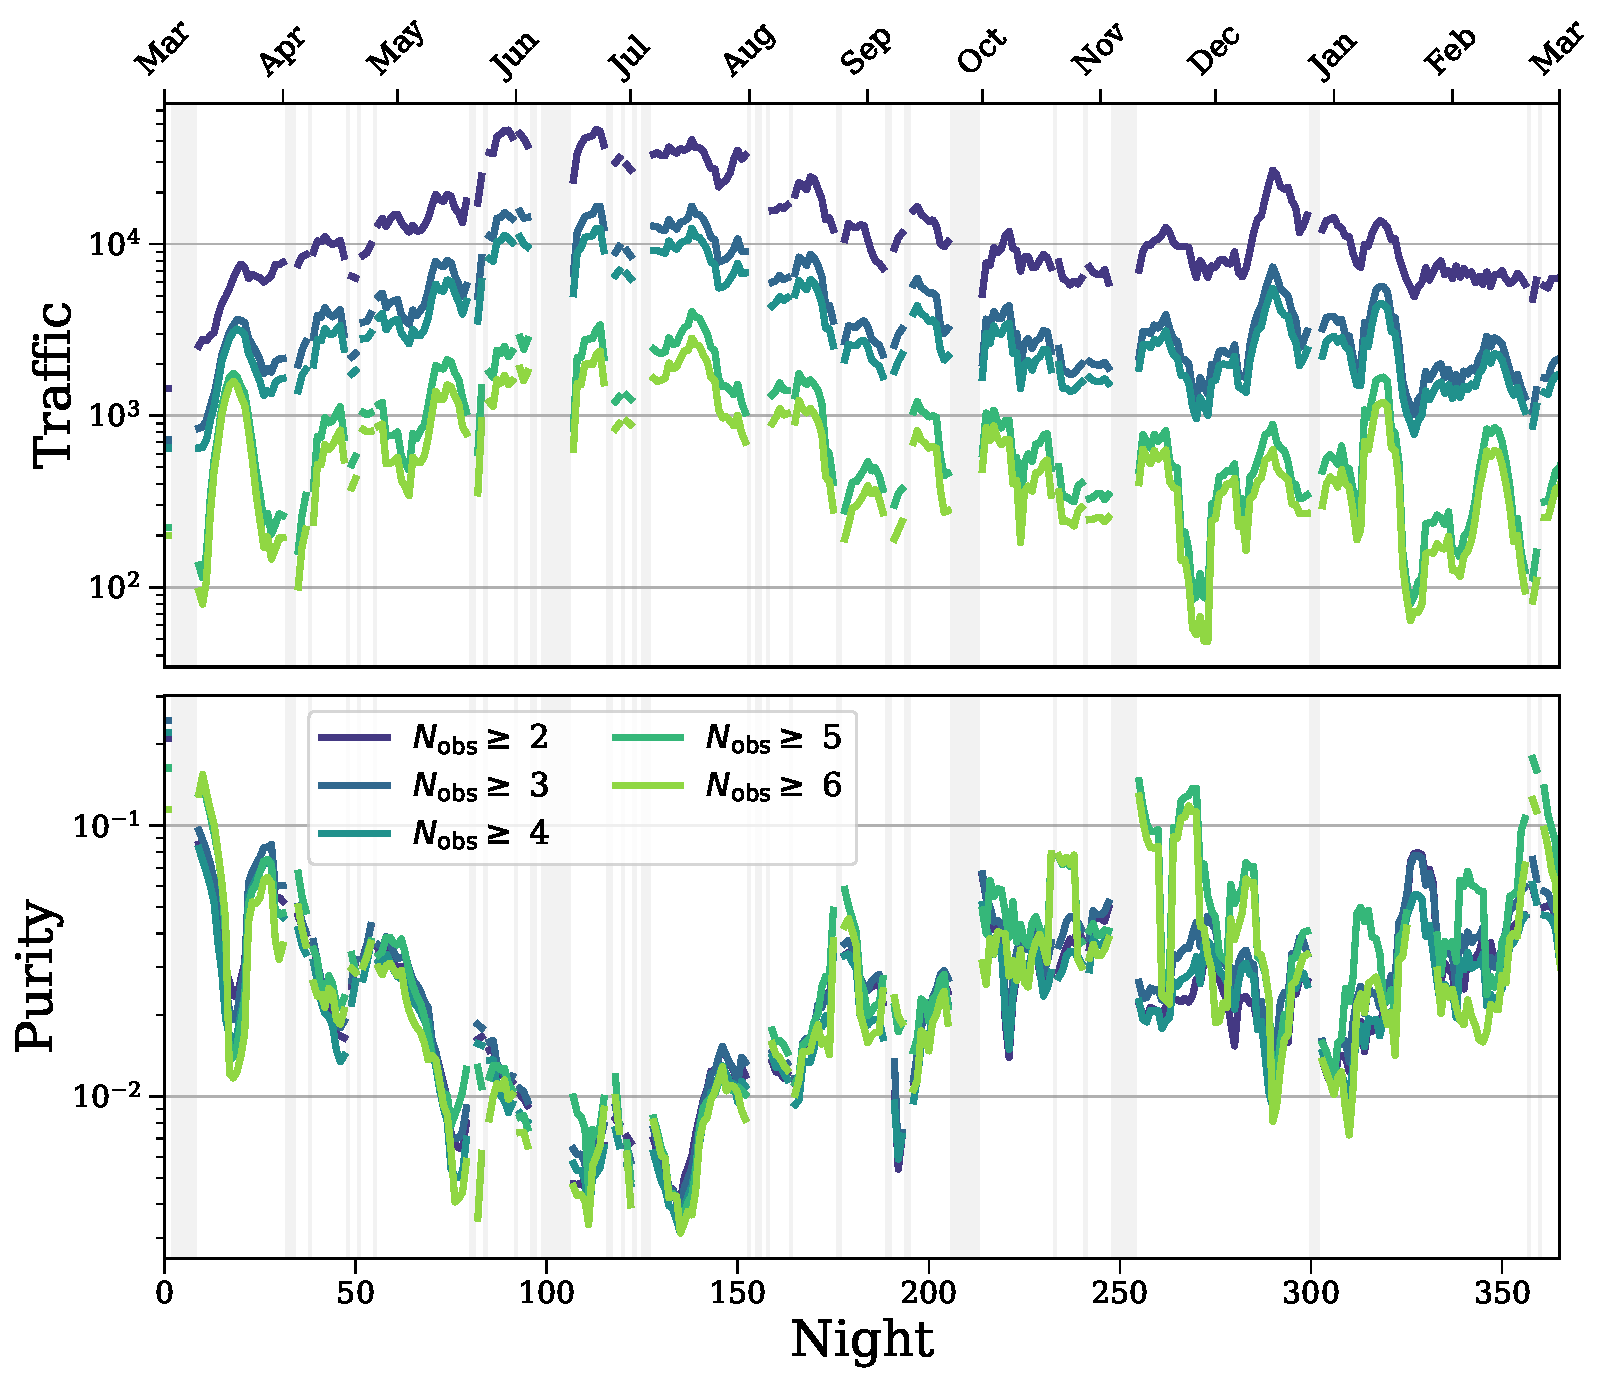
\includegraphics[width=\textwidth]{traffic_purity.pdf}
    \caption{Traffic (number of objects sent) and purity (fraction of objects sent that are NEOs) of the NEOCP during the first year of LSST if every observation that qualifies for submission is submitted. Each line is plotted using a rolling window of a week to smooth stochastic effects. Different lines correspond to different constraints on the number of observations for a tracklet to be submitted. Nights on which no observations were taken are highlighted with grey areas.}
    \label{fig:neocp_traffic}
\end{figure*}

To illustrate the performance of \dig{} on our sample, we show the distribution of \dig{} scores for the NEOs and MBAs in the first year of observations in Figure~\ref{fig:digest2_example}. As one would expect most NEOs have scores around 100, whilst most MBAs have scores around 0. However, we can already see that due to the sheer volume of MBA observations, the \dig{} score does not perform well in classifying NEOs for our sample. In particular, even an object assigned a score of 100 only has a 3\% chance of actually being an NEO. We will discuss the effect of \dig{}'s weak performance on our sample in more detail in Section~\ref{sec:discussion}.

\subsection{Traffic and Purity of NEOCP}\label{sec:traffic_basic}

\begin{figure*}
    \centering
    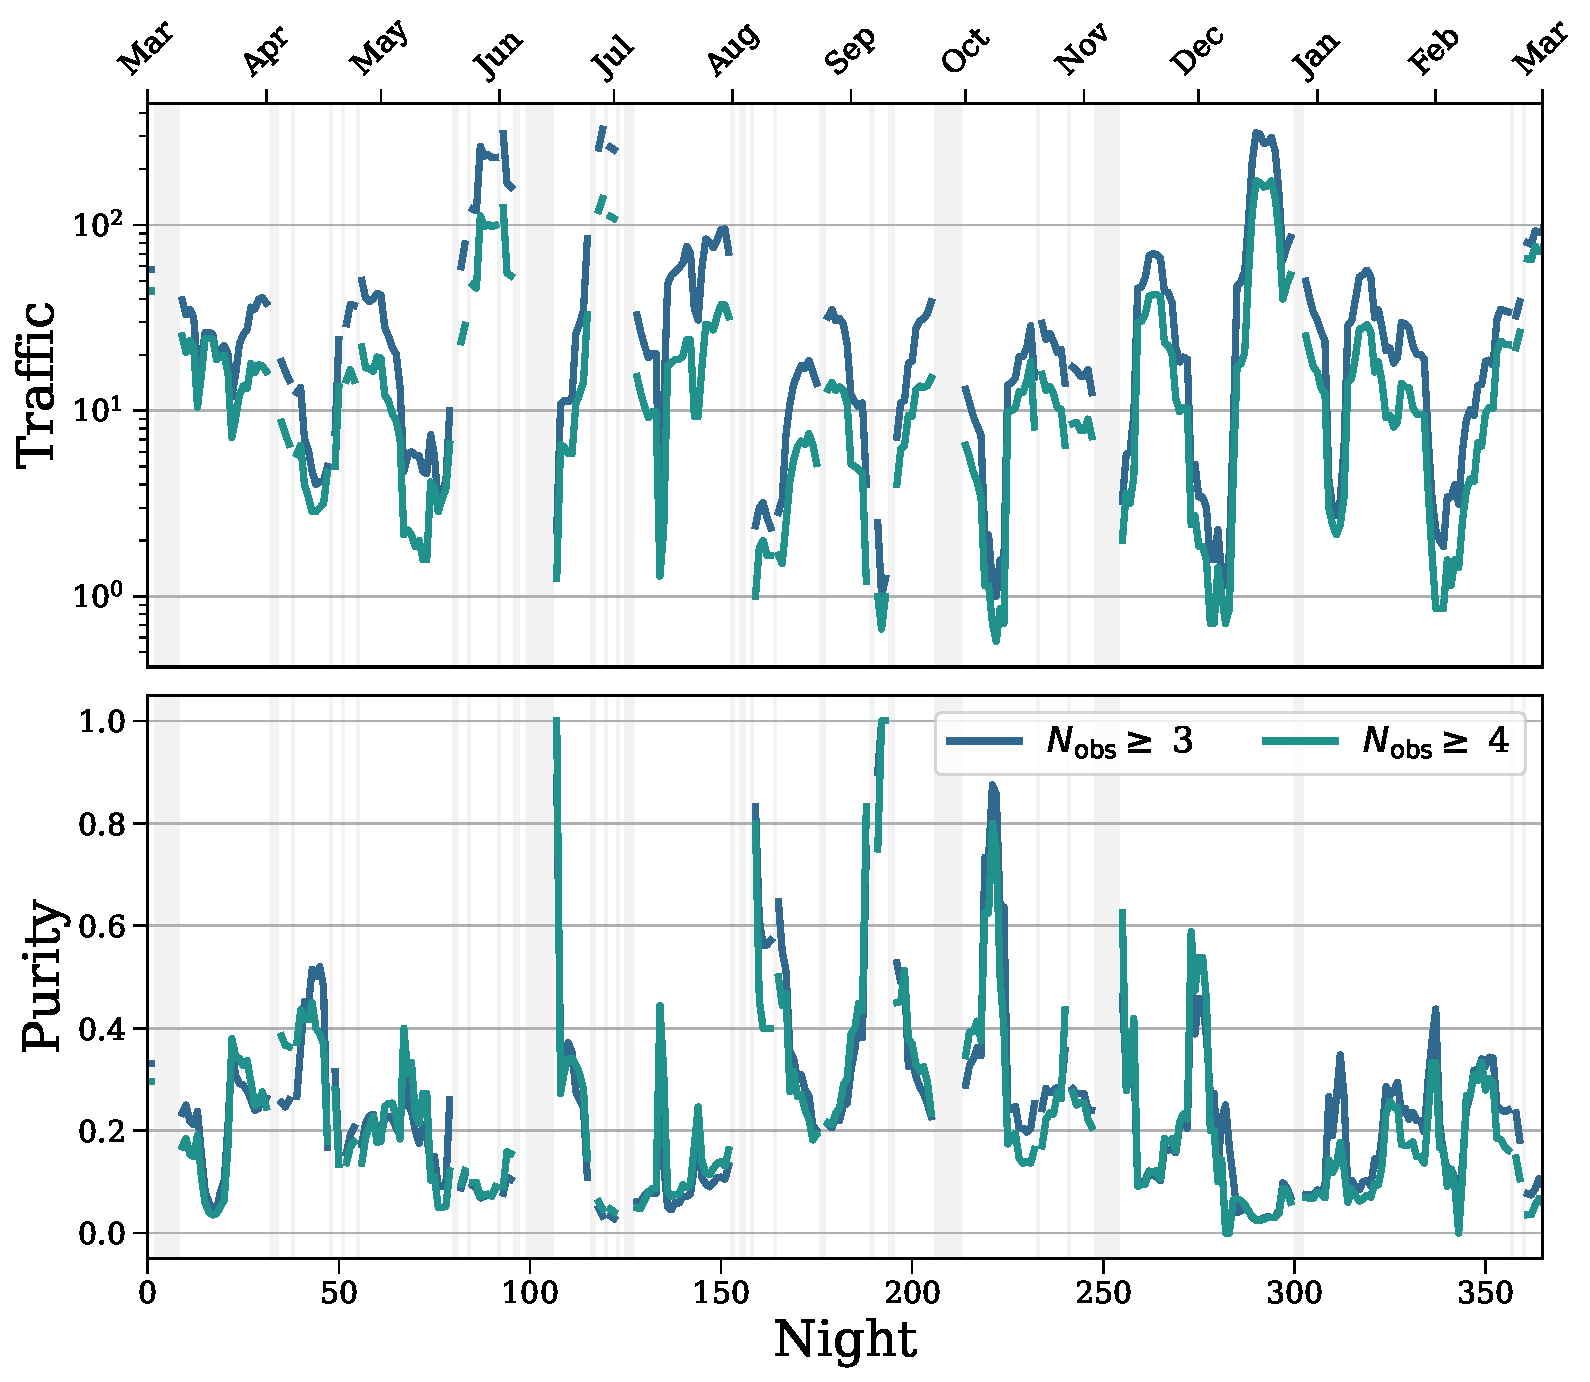
\includegraphics[width=\textwidth]{traffic_purity_unfindable.pdf}
    \caption{As Figure~\ref{fig:neocp_traffic}, but only including objects that would not be detected by LSST alone. Note the y-scale of the lower panel is now linear.}
    \label{fig:neocp_traffic_unfindable}
\end{figure*}

In Figure~\ref{fig:neocp_traffic}, we summarise the effect that LSST submissions would have on the NEOCP if \textit{every} object that met the \dig{} score criterion was submitted. The top panel shows the traffic of the NEOCP, meaning the number of objects that would be submitted to the page, whilst the bottom panel shows the purity, meaning the fraction of objects submitted to the page that are actually NEOs.

The current typical traffic of the NEOCP is on the order of two dozen new submissions per night. We show in the top panel that this traffic would increase by up to 3 orders of magnitude as a result of LSST submissions. Each line corresponding to a different number of minimum nightly observations (each increasing from the original choice of 2 as discussed in Section~\ref{sec:digest2_score}). Although the traffic is lower when requiring more observations, even when requiring a minimum of 6 observations the traffic can still reach several thousands of submissions per night, which is far more than the NEOCP is currently equipped to handle.

The purity of the NEOCP is also severely impacted by LSST observations, with the abundant MBA observations polluting the page as false NEOs. For almost the entire year the page will have a purity below 10\%, and the value reaches as low as 0.2\%. As noted in Section~\ref{sec:digest2_score}, this is due to the sheer abundance of MBAs in LSST observations. Therefore, given these purity levels a significant amount of follow-up time would be wasted in investigating MBAs masquerading as NEOs.

There are two periodic effects that can be noted in both the traffic and the purity panels. There is a clear seasonal variation over the year as the ecliptic plane moves through the sky. LSST observes from the southern hemisphere and thus in first half of the year when the ecliptic is at lower declinations, more MBAs will be observed. This both increases the traffic and decreases the purity of the NEOCP. In addition to this long term variation, there are also shorter term variations that are most clearly seen in the purity panel. On day 17 and approximately every 30 days after this there is a periodic decrease in the purity of the page. This coincides with the occurrence of a full moon, since LSST has to observe a different part of the sky during this time and this leads to more MBA detections and thus lower purity.

Overall it is clear that, if we proceed in the same manner as is currently recommended, the NEOCP will not be able to handle the load. We now consider how we could proceed differently.

\subsection{The NEOCP without LSST Detections}\label{sec:no_LSST_detections}

LSST will be able to detect and characterise many potential NEOs without any external input. This means that many of the objects submitted to the NEOCP will actually result in wasted follow-up time by the community. We assess the magnitude of this effect using the python package \texttt{difi} \citep{difi}. This package calculates which objects are detected by LSST, where a detection is defined as occurring when the same object is observed on at least 3 separate nights within a 15 day window, each with at least 2 observations separated by at most 90 minutes \citep{oss}.

In Figure~\ref{fig:neocp_traffic_unfindable}, we repeat Figure~\ref{fig:neocp_traffic}, but now only including objects that would not be detected by LSST alone. This represents a best case scenario in which we had foreknowledge of which observed objects would be detected. In this scenario we see that the traffic from LSST rarely exceeds more than 100 objects and is often only a handful. Similarly the purity is much higher, with an average of around 25\%. We conclude that if we were to know whether an object would be detected by LSST, the load on the NEOCP would remain at manageable levels. Motivated by this result, we developed the algorithm that predicts whether an object will be detected by LSST alone. We describe this algorithm and assess the effect of its application in Section~\ref{sec:mitigation}.

\section{Mitigating the impact of LSST}\label{sec:mitigation}

\subsection{Estimating LSST ``Self-follow-up'' Probability}\label{sec:pred_alg}
In choosing which objects to submit to the NEOCP from LSST, it also important to consider whether the object would be detected by LSST without external follow-up (since these objects would not need to be submitted to the NEOCP). We therefore propose a method of \textit{predicting} whether an observed object will be detected by LSST based on current observations. This requires one to predict both the location and magnitude of the object on subsequent nights, as well as the visit schedule of LSST.

In order to determine the location of an object on subsequent nights one needs to estimate its orbit. Each object on a given night consists of at least two observations, $O$, that have the form
\begin{equation}
    O = \{ \alpha, \delta, t \}
\end{equation}
where $\alpha$ is the right ascension, $\delta$ is the declination and $t$ is the time of observation. We determine the proper motion of the object on the sky, ($\dot{\alpha}$, $\dot{\delta}$), by calculating the change in position between the two observations using \texttt{Astropy SkyCoord} and dividing by the time between observations. This determines 4 of the 6 orbital elements, but the topocentric distance, $D$, and radial velocity, $\dot{D}$, of the object are unconstrained.

We draw a sample of $D$ uniformly in log-space between $[0.1, 10] \unit{AU}$ and a sample of $\dot{D}$ uniformly between $[-50, 10] \unit{km}{s^{-1}}$ to create a grid of $(D, \dot{D})$. Combining these with the measured $(\alpha, \delta, \dot{\alpha}, \dot{\delta})$ values (and adding $0.1^{\prime\prime}$ of scatter to the measured on-sky positions to account for the detector uncertainty), we create a series of possible variant orbits for the object. We back-propagate these orbits to account for the light travel time using \texttt{THOR} \citep{Moeyens+2021}. Since we are only interested in NEOs, we mask out any orbits that have a perihelion distance of greater than $1.3 \unit{AU}$. To demonstrate the different possible orbits that we could infer from a single observation, we plot a subset of the variant orbits obtained for an NEO observed in our mock observations in Figure~\ref{fig:orbits}.

\begin{figure}[htb]
    \centering
    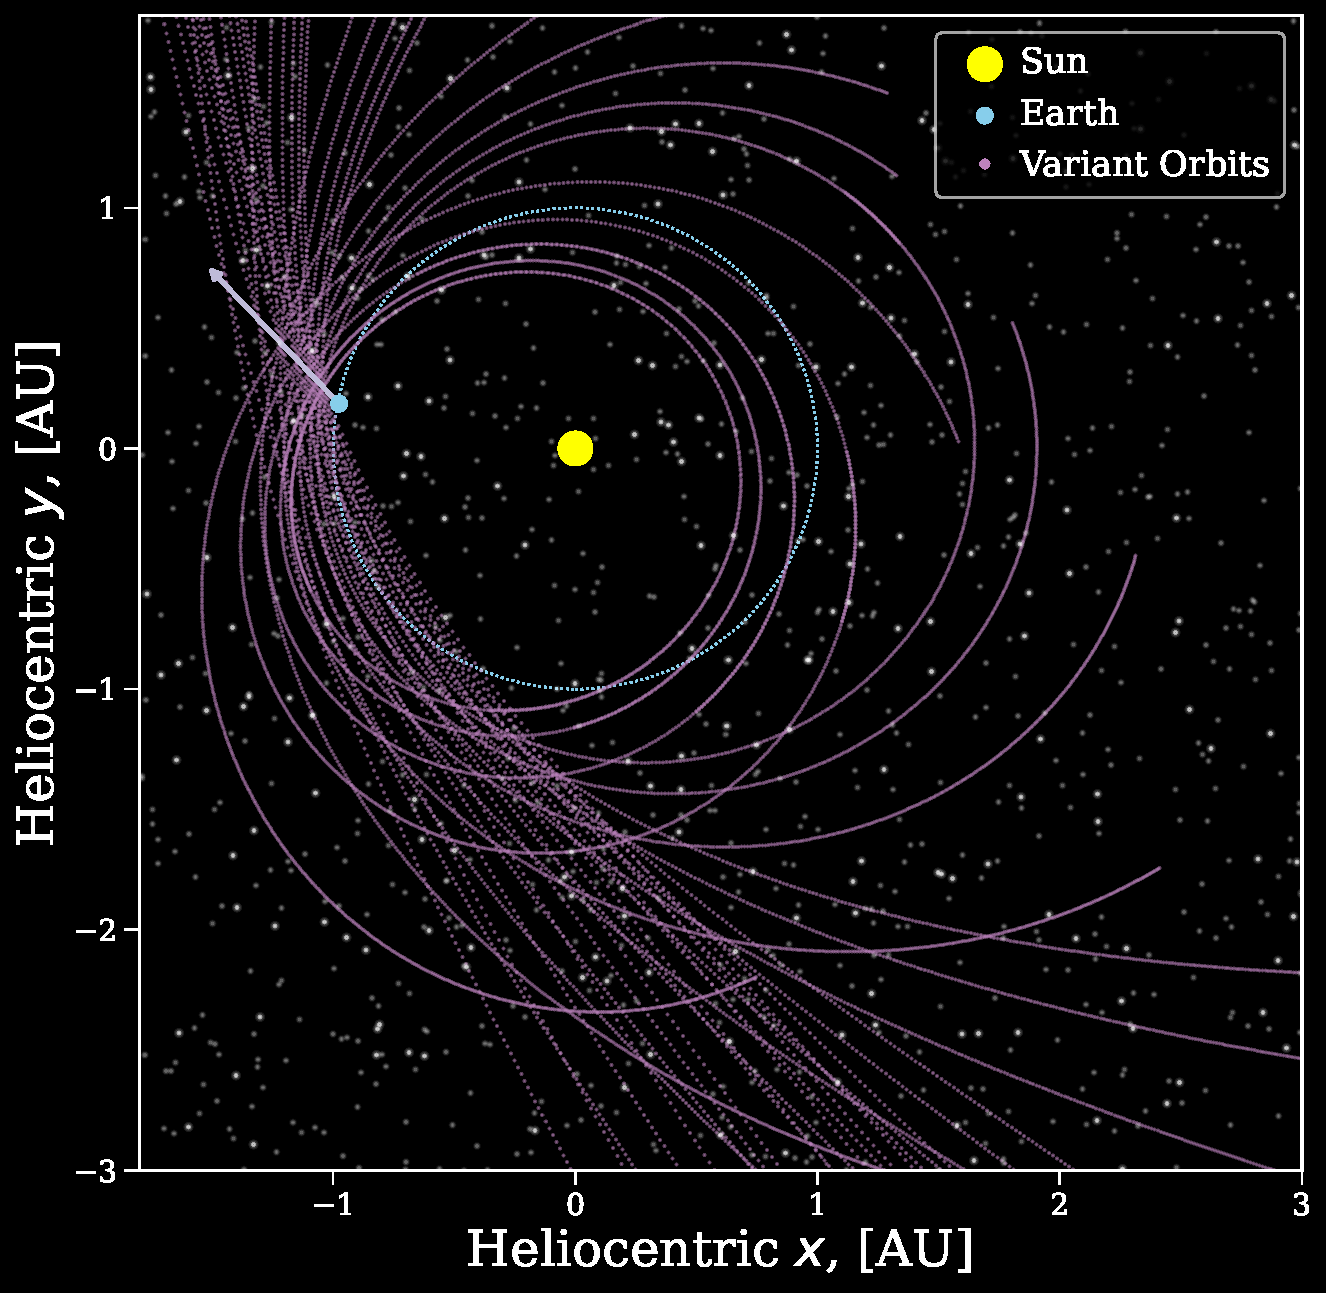
\includegraphics[width=\columnwidth]{paper/figures/orbits_example_small.pdf}
    \caption{Variant orbits that we compute for an example NEO in our sample based on a single night of mock LSST observations. The white arrow indicates the initial sight-line for the observation. The blue dotted line indicates the orbit of the Earth. Background stars are for illustrative purposes only.}
    \label{fig:orbits}
\end{figure}

% \begin{figure}[htb]
%     \centering
%     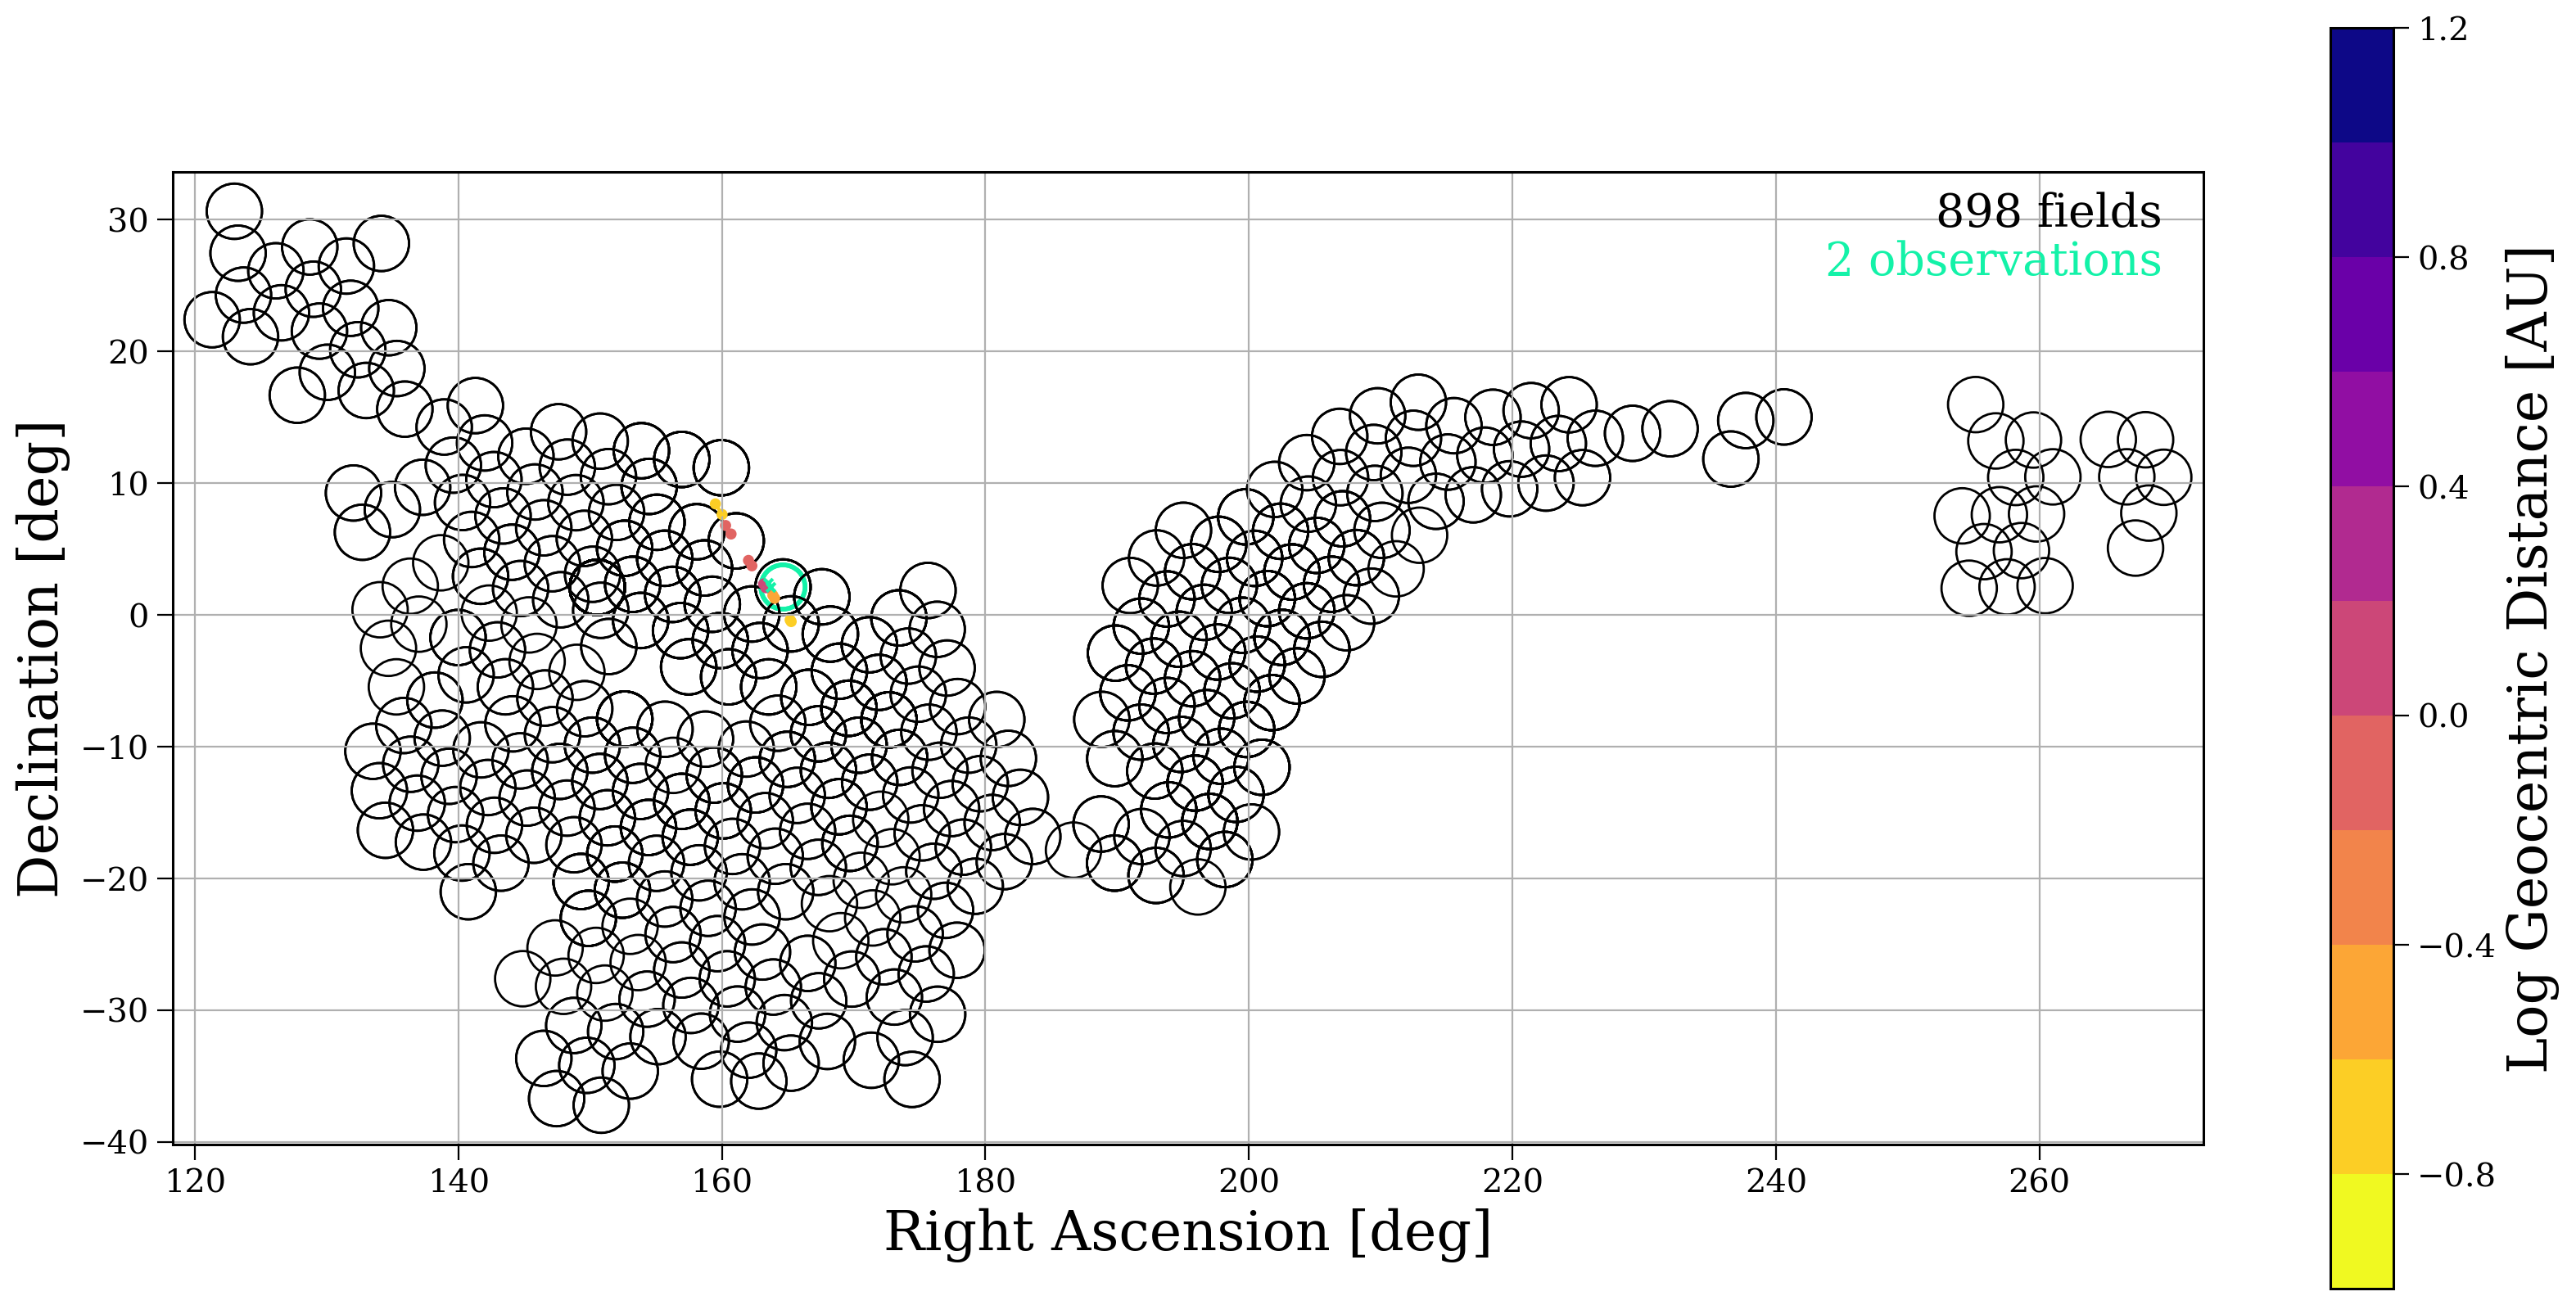
\includegraphics[width=\columnwidth]{methods_placeholder.png}
%     \caption{A demonstration of the LSST detection probability prediction. Black circles (to scale with $2.1^{\circ}$ radii) represent a bounding circle of LSST's camera footprint for each visit in this night's predicted schedule. For each orbit we plot the object's predicted location at the start and end of the night and colour them by the assumed distance. In cyan we show true position of the object and outline any visits that produce an observation in cyan also.}
%     \label{fig:circles}
% \end{figure}

Additionally, we determine the absolute magnitude of the object for each orbit using the $HG$-system \citep{mpc_h_g}. We use the LSST colour definitions, assuming a C-type asteroid, to convert the apparent magnitudes of the initial observations to V-band magnitudes \citep{Jones+2018}. We additionally calculate the phase angle of the asteroid, $\alpha$, as
\begin{equation}
    \cos \alpha = \frac{D_{a, \odot}^2 + D_{a, \oplus}^2 - D_{\odot, \oplus}^2}{2 D_{a, \odot}^2 D_{a, \oplus}^2}
\end{equation}
where $D_{a, \odot}$ is the distance between the asteroid and the Sun, $D_{a, \oplus}$ is the distance between the asteroid and the Earth and $D_{\odot, \oplus}$ is the distance from the Sun to the Earth. We then use the mean observed V-band magnitude, the assumed distances, the phase angle and a fixed slope parameter of $G = 0.15$ (as is customary) to calculate the current absolute magnitude \citep{mpc_h_g}.

For each night in the first year, we use \texttt{rubin\_sim} to create a predicted schedule for the following 14 nights, our assumed detection window \citep{rubin_sim}. These predicted schedules represent an estimate of where LSST will look next and as such account for scheduled downtime, but do not include unscheduled downtime or poor weather conditions. This means the predicted schedule may include visits on nights where no observations were possible or that the reduced seeing means that fainter objects would be missed.

Finally, using \texttt{OpenOrb}, we produce ephemerides for the orbits for each visit in the following 14 nights of the predicted schedule that the object could potentially reach based on its observed on-sky motion \citep{Granvik+2009}. For each orbit and each field, we check whether the object is within the LSST camera footprint of the field using \texttt{rubin\_sim} \citep{rubin_sim}. We additionally convert the predicted apparent magnitude back to the relevant filter and assess whether the object has an apparent magnitude brighter than the $5\sigma$ depth of field. If both of these criteria are met then we assume an observation has been made.

Each orbit is defined as producing a detection if it has at least 3 observations on at least 3 nights in a 15 day window, requiring that the minimum arc length is 1 arcsecond and that the maximum separation between observations is 90 minutes \citep{oss}. We additionally account for all prior observations in this calculation. For example, if we were determining the probability of detection for an object that is observed on night 10 and has previously been observed on night 8, even if we only predict that it will be observed on night 14 in the next 15 days, this would still be deemed a detection. We estimate the overall probability of the object being detected by LSST as a simple fraction of orbits that produce detections.



\subsection{Using the LSST detection probability algorithm}\label{sec:using_alg}

\begin{figure*}[htb]
    \centering
    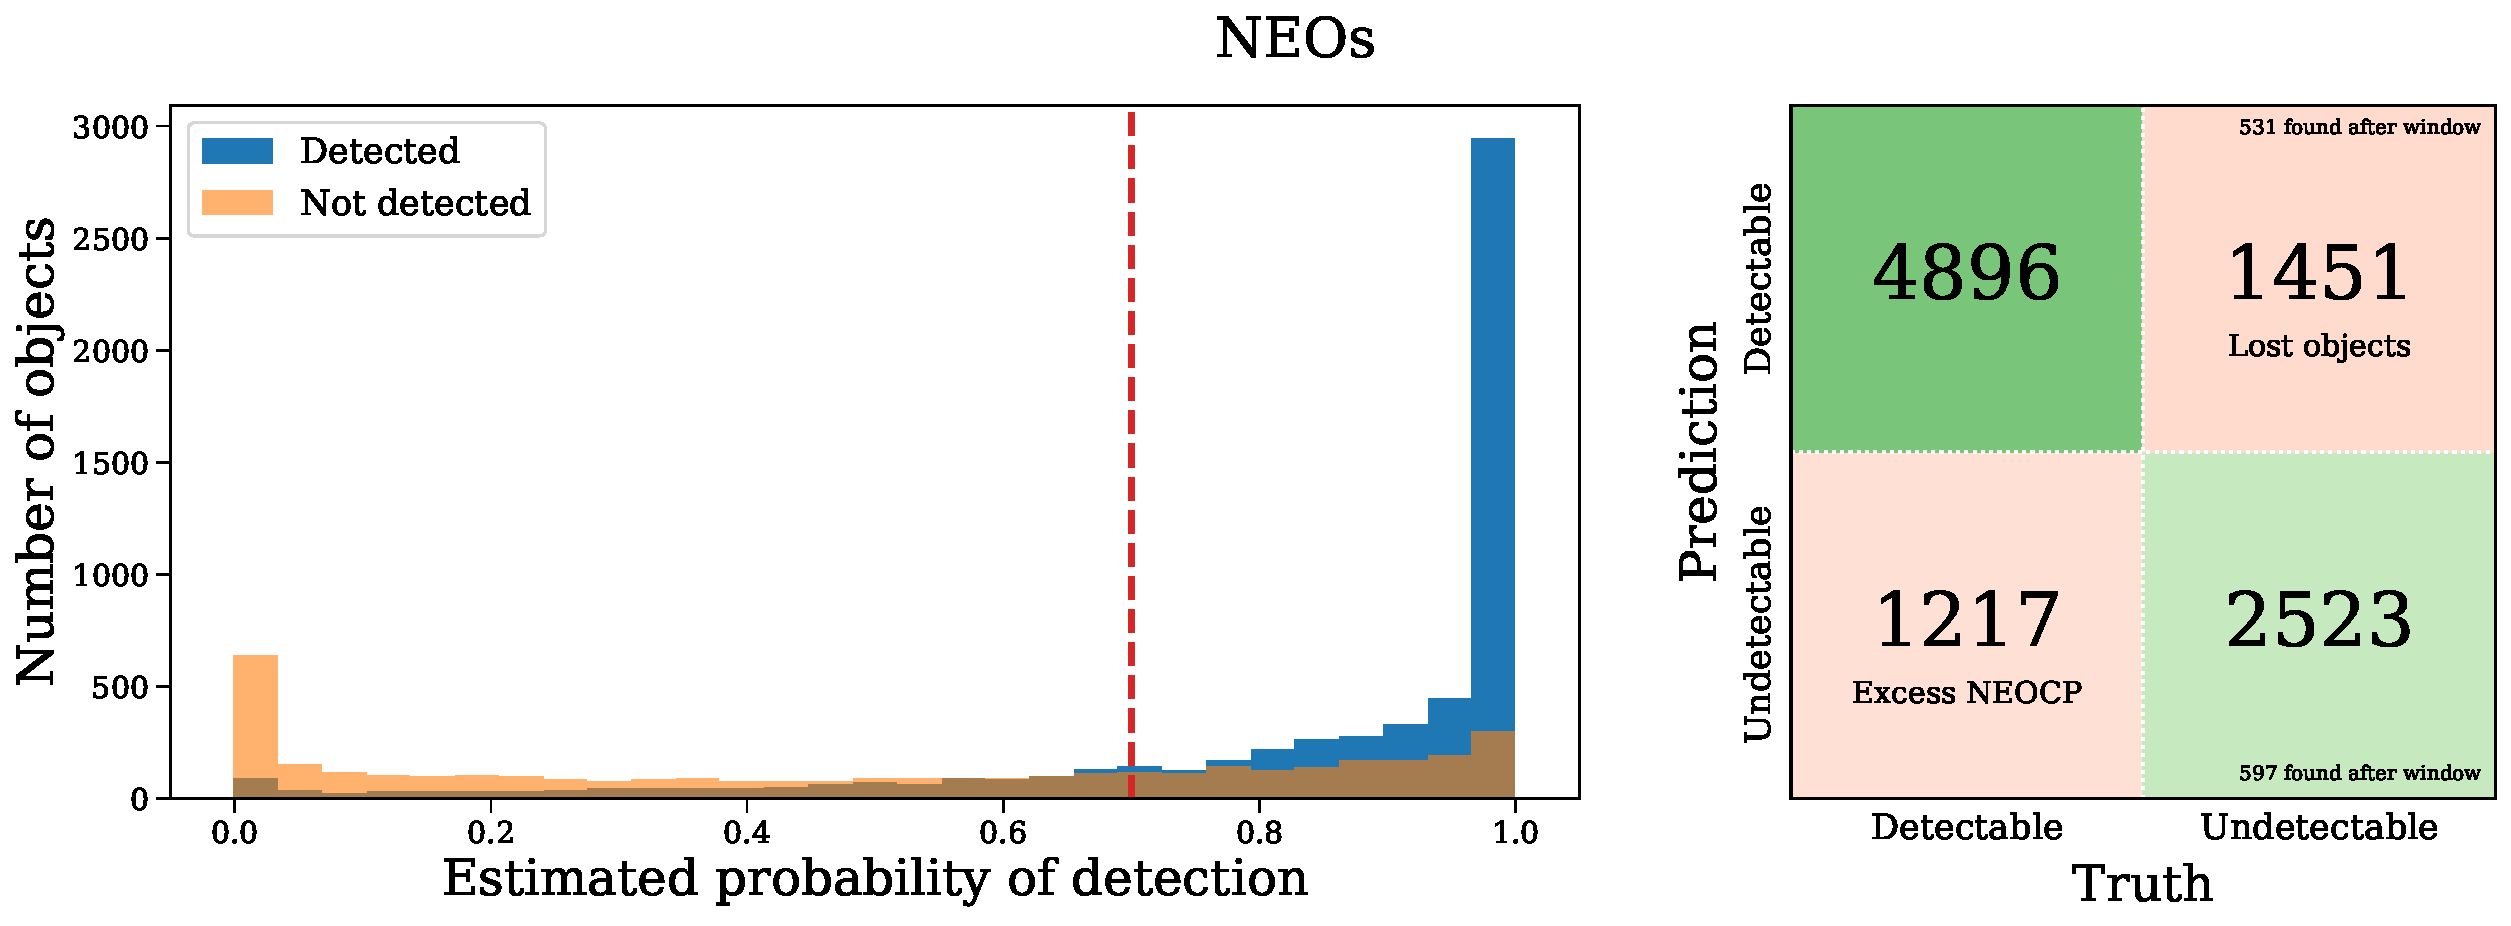
\includegraphics[width=\textwidth]{contingency_neo.pdf}
    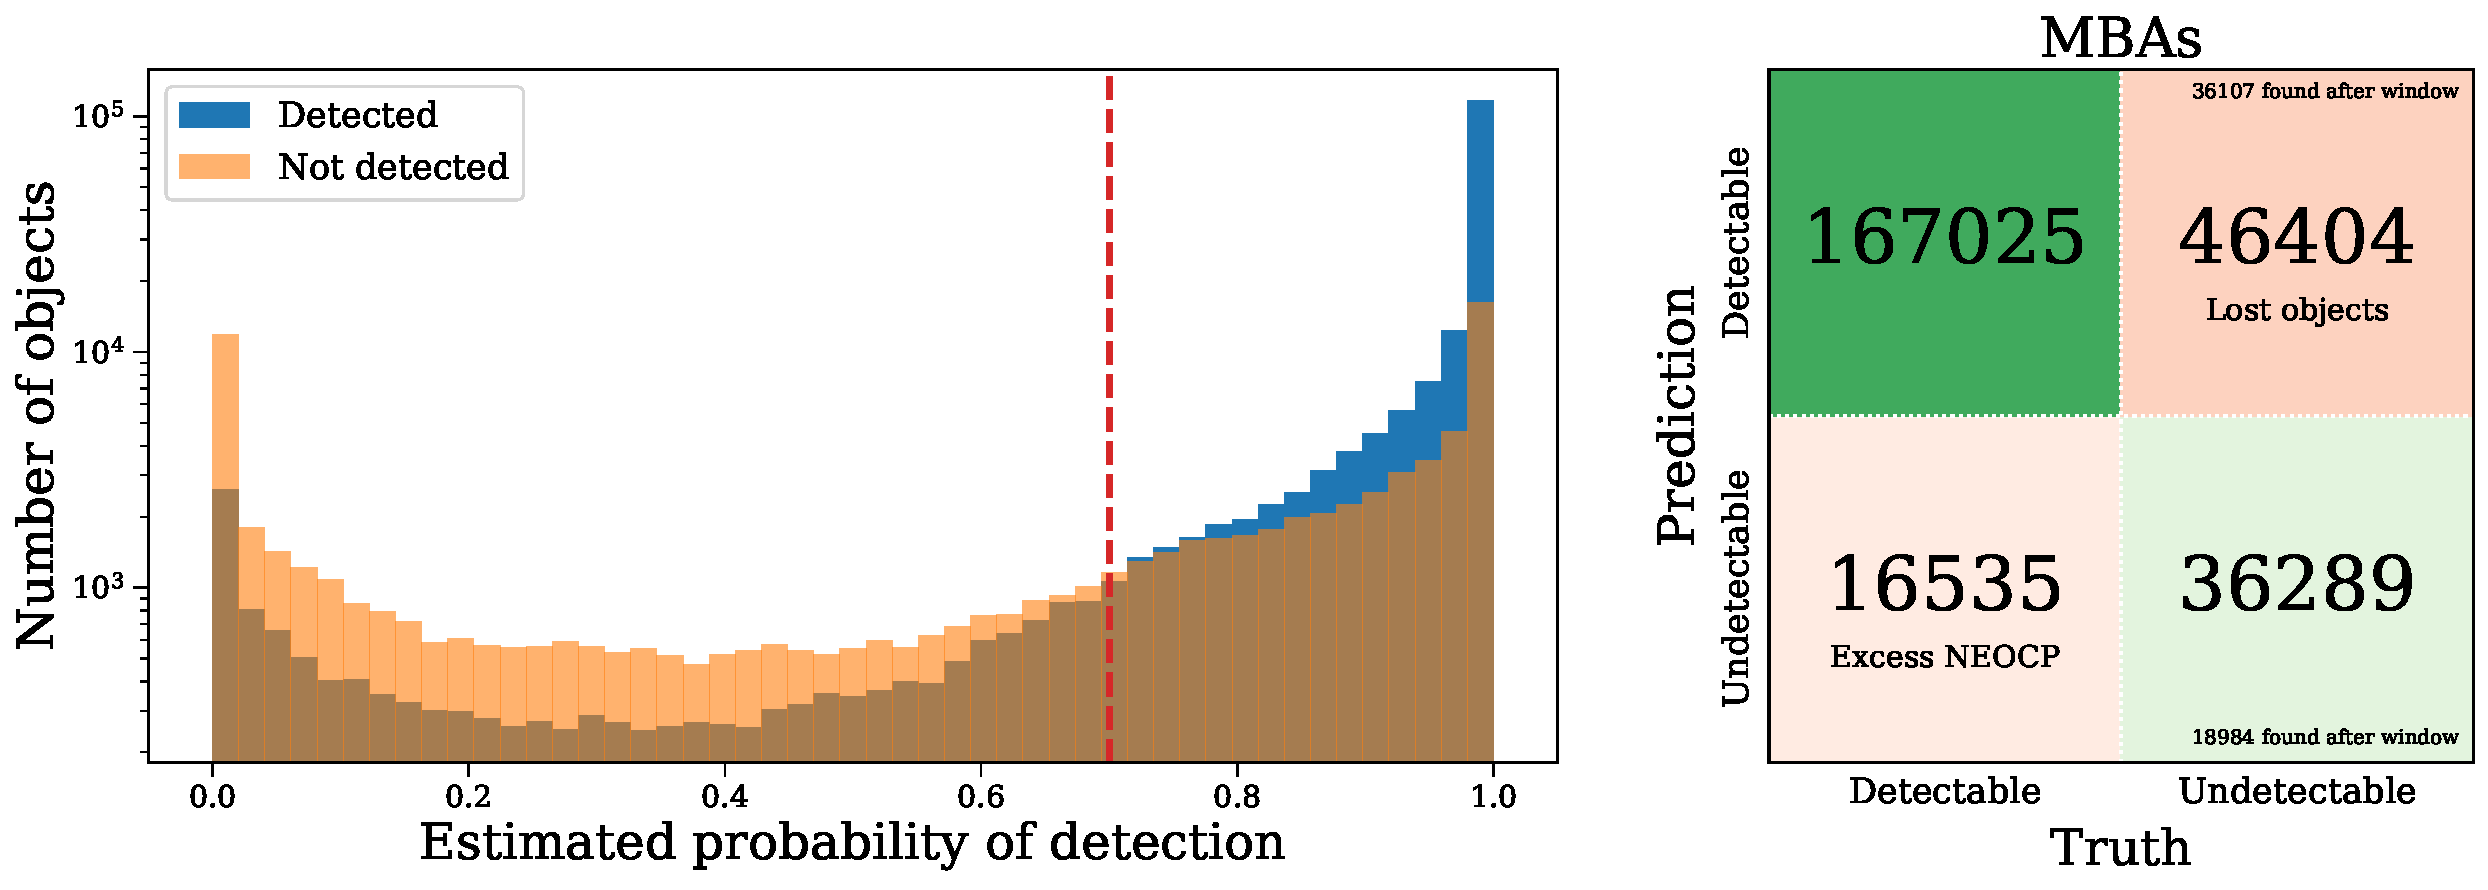
\includegraphics[width=\textwidth]{contingency_mba.pdf}
    \caption{A demonstration of the prediction algorithm described in Section~\ref{sec:pred_alg} using 1 year of simulated observations for both NEOs (top) and MBAs (bottom). \textbf{Left:} Probability that an object will be detected within 15 nights, split into a population of objects that are \textit{actually} detected within 15 nights in the simulated observations and a population that are not. The red dashed line indicates our threshold of $\thresholdAlg{}$ for submission to the NEOCP. Note that the histogram is on a logarithmic scale for the MBAs. \textbf{Right:} A contingency matrix representing the algorithm's ability to predict the detectability of an object.}
    \label{fig:contingency}
\end{figure*}
We now examine the effect of applying the LSST detection probability algorithm to reduce the load on the NEOCP. Figure~\ref{fig:contingency} shows the results for a year of simulated observations for both the NEOs and MBAs. The histograms show the estimated probability of detection by LSST for each object, split into a population of objects that are \textit{actually} detected within 15 nights in our simulated observations and a population that are not. On average the algorithm predicts the correct outcome approximately $\efficiencyAlg{}\%$ of the time.

We use a threshold of $\thresholdAlg{}$ for deciding whether an object will be detected by LSST (and therefore whether to submit it to the NEOCP). We found that this value was ideal for minimising the number of NEOs that are lost and the number of objects sent to the NEOCP, whilst maximising the fraction of those objects that are NEOs.

In the right side of Figure~\ref{fig:contingency}, we show contingency matrices for both NEOs and MBAs when applying this threshold. The lower left quadrants give a count of the number of objects that will be sent to the NEOCP needlessly as LSST will detect them without follow-up. The upper right quadrants total the number of objects that will be lost, since LSST will not detect them within the given detection window but they would also not be sent to the NEOCP. We additionally annotate the number of objects that would be found after the detection window and note this reduces the overall number of lost objects.

Overall, when applying this threshold, we find that, on average, $\npernightAlg{}$ objects would be submitted to the NEOCP per night, but only around $\purityAlg{}\%$ (${\sim}\purityAlgRaw{}$) of those objects would be NEOs. Moreover, $\neoLostAlg{}$ NEOs would remain undetected by LSST and not be sent to the NEOCP for follow-up. This method would reduce the traffic on the NEOCP by more than an order of magnitude, however there is only a small improvement on the purity of the submitted objects and the vast majority of submissions would still be MBAs. 

\section{Discussion} \label{sec:discussion}
As we have shown above, even when applying our LSST detection probability algorithm, the NEOCP would be overwhelmed by submissions from LSST and significantly more MBAs would be submitted than NEOs. In this section we consider recommendations for how to mitigate these issues and ensure that the NEOCP remains functional in the era of LSST.

\subsection{Improve \dig{} algorithm}
In Figure~\ref{fig:digest2_example} we highlighted that \dig{} struggles to distinguish between NEOs and MBAs when dealing with the extreme volumes of MBAs that LSST will observe. When using the first year of simulated LSST observations, we find that only ${\sim}1.5\%$ of objects with a \dig{} NEO score of at least 65 (the threshold for submission to the NEOCP) are in fact NEOs.

For this reason, it is important to consider whether there are improvements that can be made to the \dig{} algorithm in distinguishing between NEOs and MBAs. Given the required suppression factor for MBAs and extensive prior work done on this algorithm, it is unlikely that such improvements would be able to eliminate this problem in all regimes. However, it is possible that there are still particular cases or particular areas of the sky in which the distinction would be improved. For instance, the algorithm could take into account the location of the ecliptic at the time of observations and penalise the NEO score of objects that are particularly close to the ecliptic.

\subsection{Await reduced MBA background}
The main problem currently stems from the abundance of MBAs relative to NEOs. We expect that after the first year of observations LSST will discover approximately $85\%$ of all MBAs down to its flux limit \citep{Juric+2020}. This will strongly suppress the number of MBAs that would submitted to the NEOCP.

At the same time, we expect a significant fraction of NEOs to be smaller objects that come for infrequent close approaches and so, even with new detections, we still expect a constant flux of new NEOs \citep{Juric+2020}. In this way the number of NEOs that are submitted to the page would remain roughly constant.

Therefore, once most of the MBAs have been identified, the traffic and purity of NEOCP submissions from LSST would be significantly improved. Indeed, when applying our LSST detection probability algorithm in addition, we expect that the resulting traffic and purity would approximate the ideal case described in Section~\ref{sec:no_LSST_detections}.

The disadvantage of this approach of course is that one would need to wait until the first year of observations were complete. This means that any NEOs that will not be re-observed after the first year would not be sent for follow-up and may be lost.

\section{Summary \& Conclusions} \label{sec:conclusion}
We present new predictions for the NEOCP in the era of LSST. We performed mock LSST observations and used \dig{} to estimate the number of objects that LSST would send to the NEOCP using the current criteria. We created a new algorithm for predicting whether an object will be detected by LSST without external follow-up based on a single night of observations in order to reduce the load on the NEOCP. Our main conclusions can be summarised as:

\begin{enumerate}
    \item \textbf{The NEOCP would be overwhelmed by LSST using current submission criteria}\\We show that the traffic (number of objects submitted) and purity (fraction of objects that are NEOs) of the NEOCP will be severely impacted by LSST. In particular, the traffic will increase by over two orders of magnitude to between 1000-20000 objects per night, whilst the purity would range from 0.2\%-10\% (Section~\ref{sec:traffic_basic}).
    \item \textbf{We present an algorithm that would reduce the impact of LSST on the NEOCP, though not fully solve the problem}\\The application of our LSST detection prediction algorithm would reduce the traffic back to reasonable levels of approximately ${\sim}\npernightAlg{}$ objects per night. However the purity still remains at an average of $\purityAlg{}\%$ due to the large MBA background (Section~\ref{sec:using_alg}).
    \item \textbf{NEO follow-up from LSST should not be attempted in the first year}\\Due to the vast number of MBA observations in the first year we recommend that follow-up should not be attempted until the second year. At this point around $85\%$ of MBAs will have been identified, whilst the rate of NEO observations will remain roughly constant and so the purity of NEOCP submissions from LSST would return to reasonable levels when using our algorithm (Section~\ref{sec:discussion}).
\end{enumerate}

\begin{acknowledgements}
    We thank Aren Heinze, Pedro Bernardenelli, Andy Connolly and Stephen Portillo for insightful discussions. We also thank Jessica Werk and Eric Agol for helpful feedback on an initial draft of this work.
\end{acknowledgements}

\software{\dig{} v0.19.2 \citep{Keys+2019}, \texttt{OpenOrb} \citep{Granvik+2009}, \texttt{difi} \citep{difi}, \texttt{THOR} \citep{Moeyens+2021}, \texttt{rubin\_sim} \citep{rubin_sim}, \texttt{Astropy} \citep{astropy:2013, astropy:2018, astropy:2022}, \texttt{astroML} \citep{VanderPlas+2012,VanderPlas+2014}, \texttt{Python} \citep{python}, \texttt{numpy} \citep{numpy}, \texttt{pandas} \citep{pandas_1.4.2, pandas_paper}, \texttt{matplotlib} \citep{matplotlib}, \texttt{scipy} \citep{Virtanen+2020}}

\bibliographystyle{aasjournal}
\bibliography{paper}{}

\restartappendixnumbering

\allowdisplaybreaks
\appendix

\section{Hybrid Catalogue Pipeline}\label{app:hybrid}
Many studies that make predictions for LSST use a synthetic catalogue of solar system objects that doesn't account for prior observations. In reality, we have already detected more than a million objects in the solar system and this number will continue to grow until LSST comes online. This means that, current predictions of detection rates will be inflated since a fraction of ``new'' detections may already be known. Therefore, for this paper we created ``hybrid'' catalogue that combines a synthetic catalogue with all known observations, whilst keeping the population distributions relatively unchanged.

We created the hybrid catalogue to be dynamic, such that we can run a single pipeline to merge in an updated version of \mpco{} as more objects are discovered in the time until LSST comes online. All code to reproduce this hybrid catalogue is open-source and available on GitHub\footnote{\url{https://github.com/dirac-institute/hybrid_sso_catalogue/tree/main/hybridcat/hybridcat}}.

\subsection{Data preprocessing}
For the synthetic catalogue of the solar system with we use \sss{}, the Pan-STARRS Synthetic Solar System Model \citep[\sss{}][]{Grav+2011}. We merge this synthetic catalogue with the latest version of \mpco{}\footnote{\url{https://minorplanetcenter.net//iau/MPCORB.html}}, a database of all currently known objects. We use \texttt{OpenOrb} \citep{Granvik+2009} to convert both catalogues to Cartesian coordinates and propagate all orbits until the same date.

\subsection{Merging algorithm}
The general idea for the merging algorithm is to inject each object from \mpco{} into \sss{}, replacing objects that are similar to those injected. An object's similarity is determined based on its position, $\va{x}$, velocity, $\va{v}$, and absolute magnitude (size), ${H}$.

We split each catalogue into bins of absolute magnitude linearly spaced from $-2$ to $28$ and perform the merge algorithm on each bin separately. For each bin we build a K-D trees for both catalogues based on the positions ($x, y, z$) of objects. For every \mpco{} object we query the \sss{} tree for the nearest $100$ objects up to a maximum distance of $0.1 \unit{AU}$, excluding any that have already been matched to a different real object. From these remaining nearest neighbours, we select the \sss{} object with the closest velocity as the matched object. If there were no remaining neighbours, either because no synthetic objects were nearby or because all nearby objects had already been matched, then we directly add this real object without replacing a synthetic one.

To complete the merging process, we compile the matched object IDs and delete them from \sss{}. We then add the entirety of \mpco{} to the remaining catalogue, resulting in a hybrid catalogue.

\subsection{Assessing quality of hybrid catalogue}\label{app:hybrid_quality}
It is essential that the underlying distributions of the hybrid catalogue do not differ significantly from \sss{} so that we still accurately reproduce the solar system. In Figure~\ref{fig:hybrid_vs_s3m_dists}, we show the distributions of the absolute magnitude and six orbital elements in both the hybrid catalogue and \sss{}. It is evident that the distributions are essentially identical.

As a further check, we compared \mpco{} to the objects that were removed from \sss{}, since these should have nearly identical distributions other than MPCORB objects that had no matches. In Figure~\ref{fig:density_compare}, we show a comparison of the densities for the heliocentric $x$ and $y$ and it is clear that these distributions are left unchanged in the hybrid catalogue.
\begin{figure*}[htb]
    \centering
    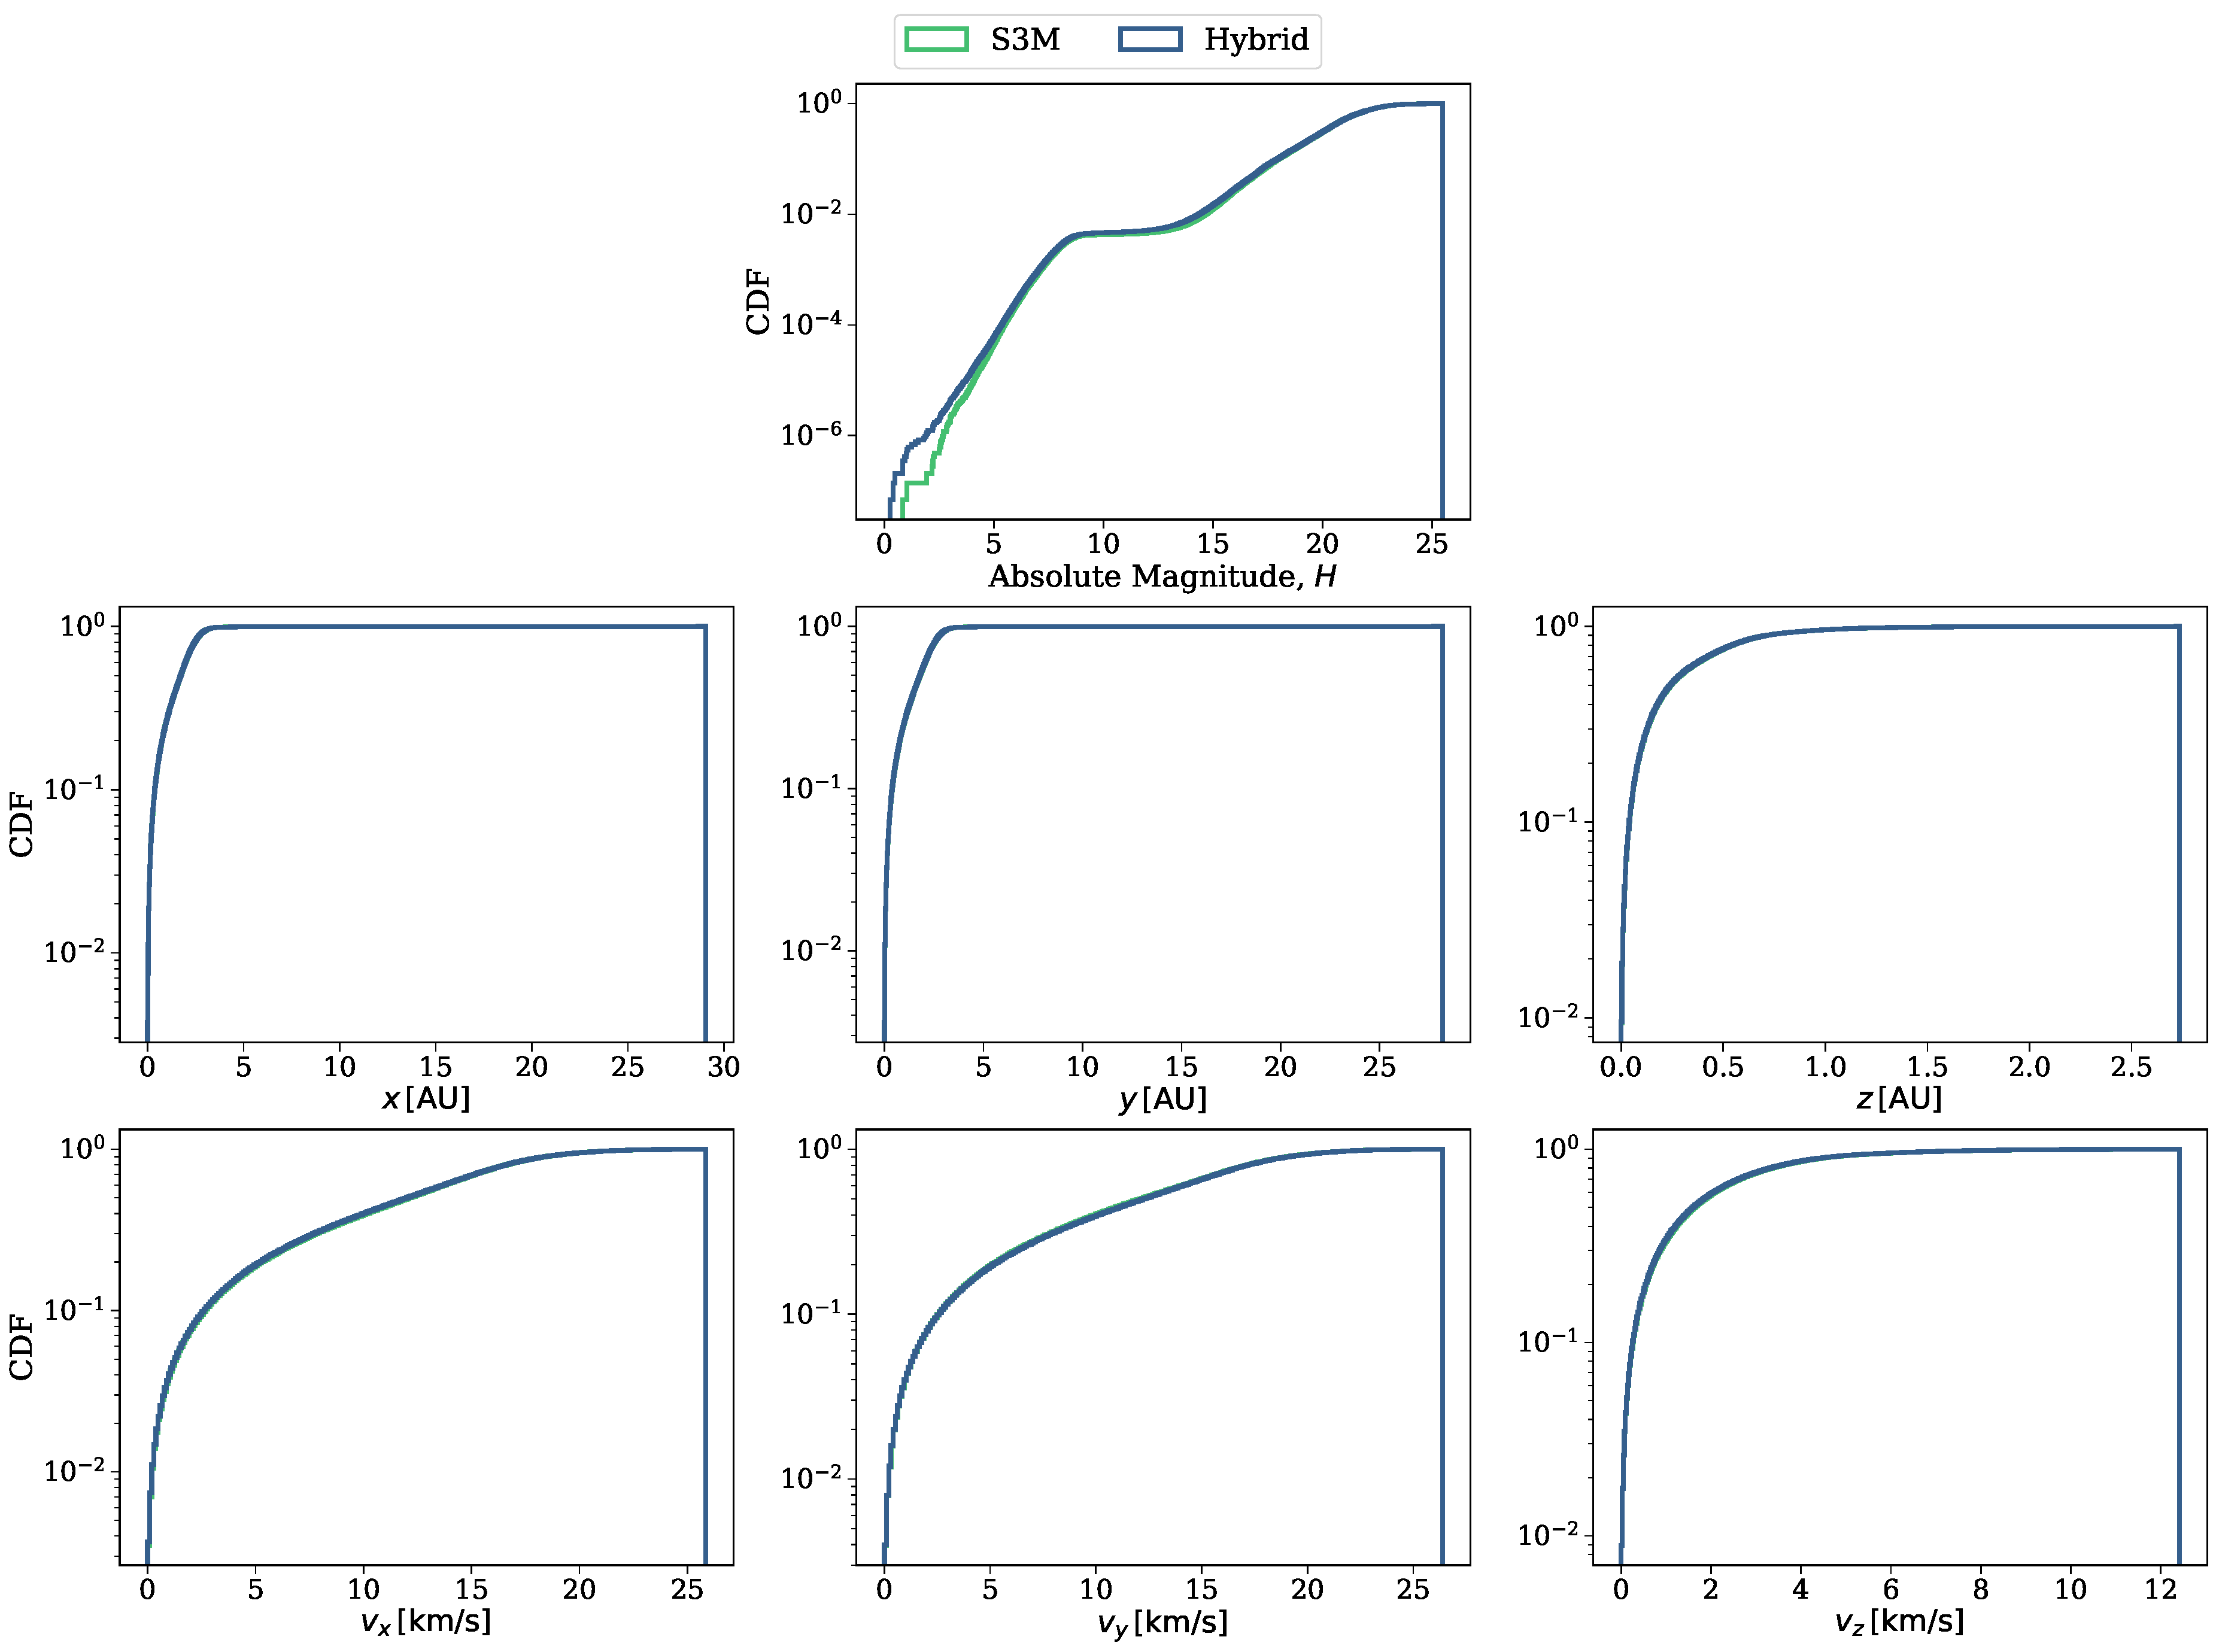
\includegraphics[width=\textwidth]{hybrid_vs_s3m_distributions.pdf}
    \caption{A comparison of the parameter distributions of \sss{} \citep{Grav+2011} and the hybrid catalogue we created.}
    \label{fig:hybrid_vs_s3m_dists}
\end{figure*}
\begin{figure}[htb]
    \centering
    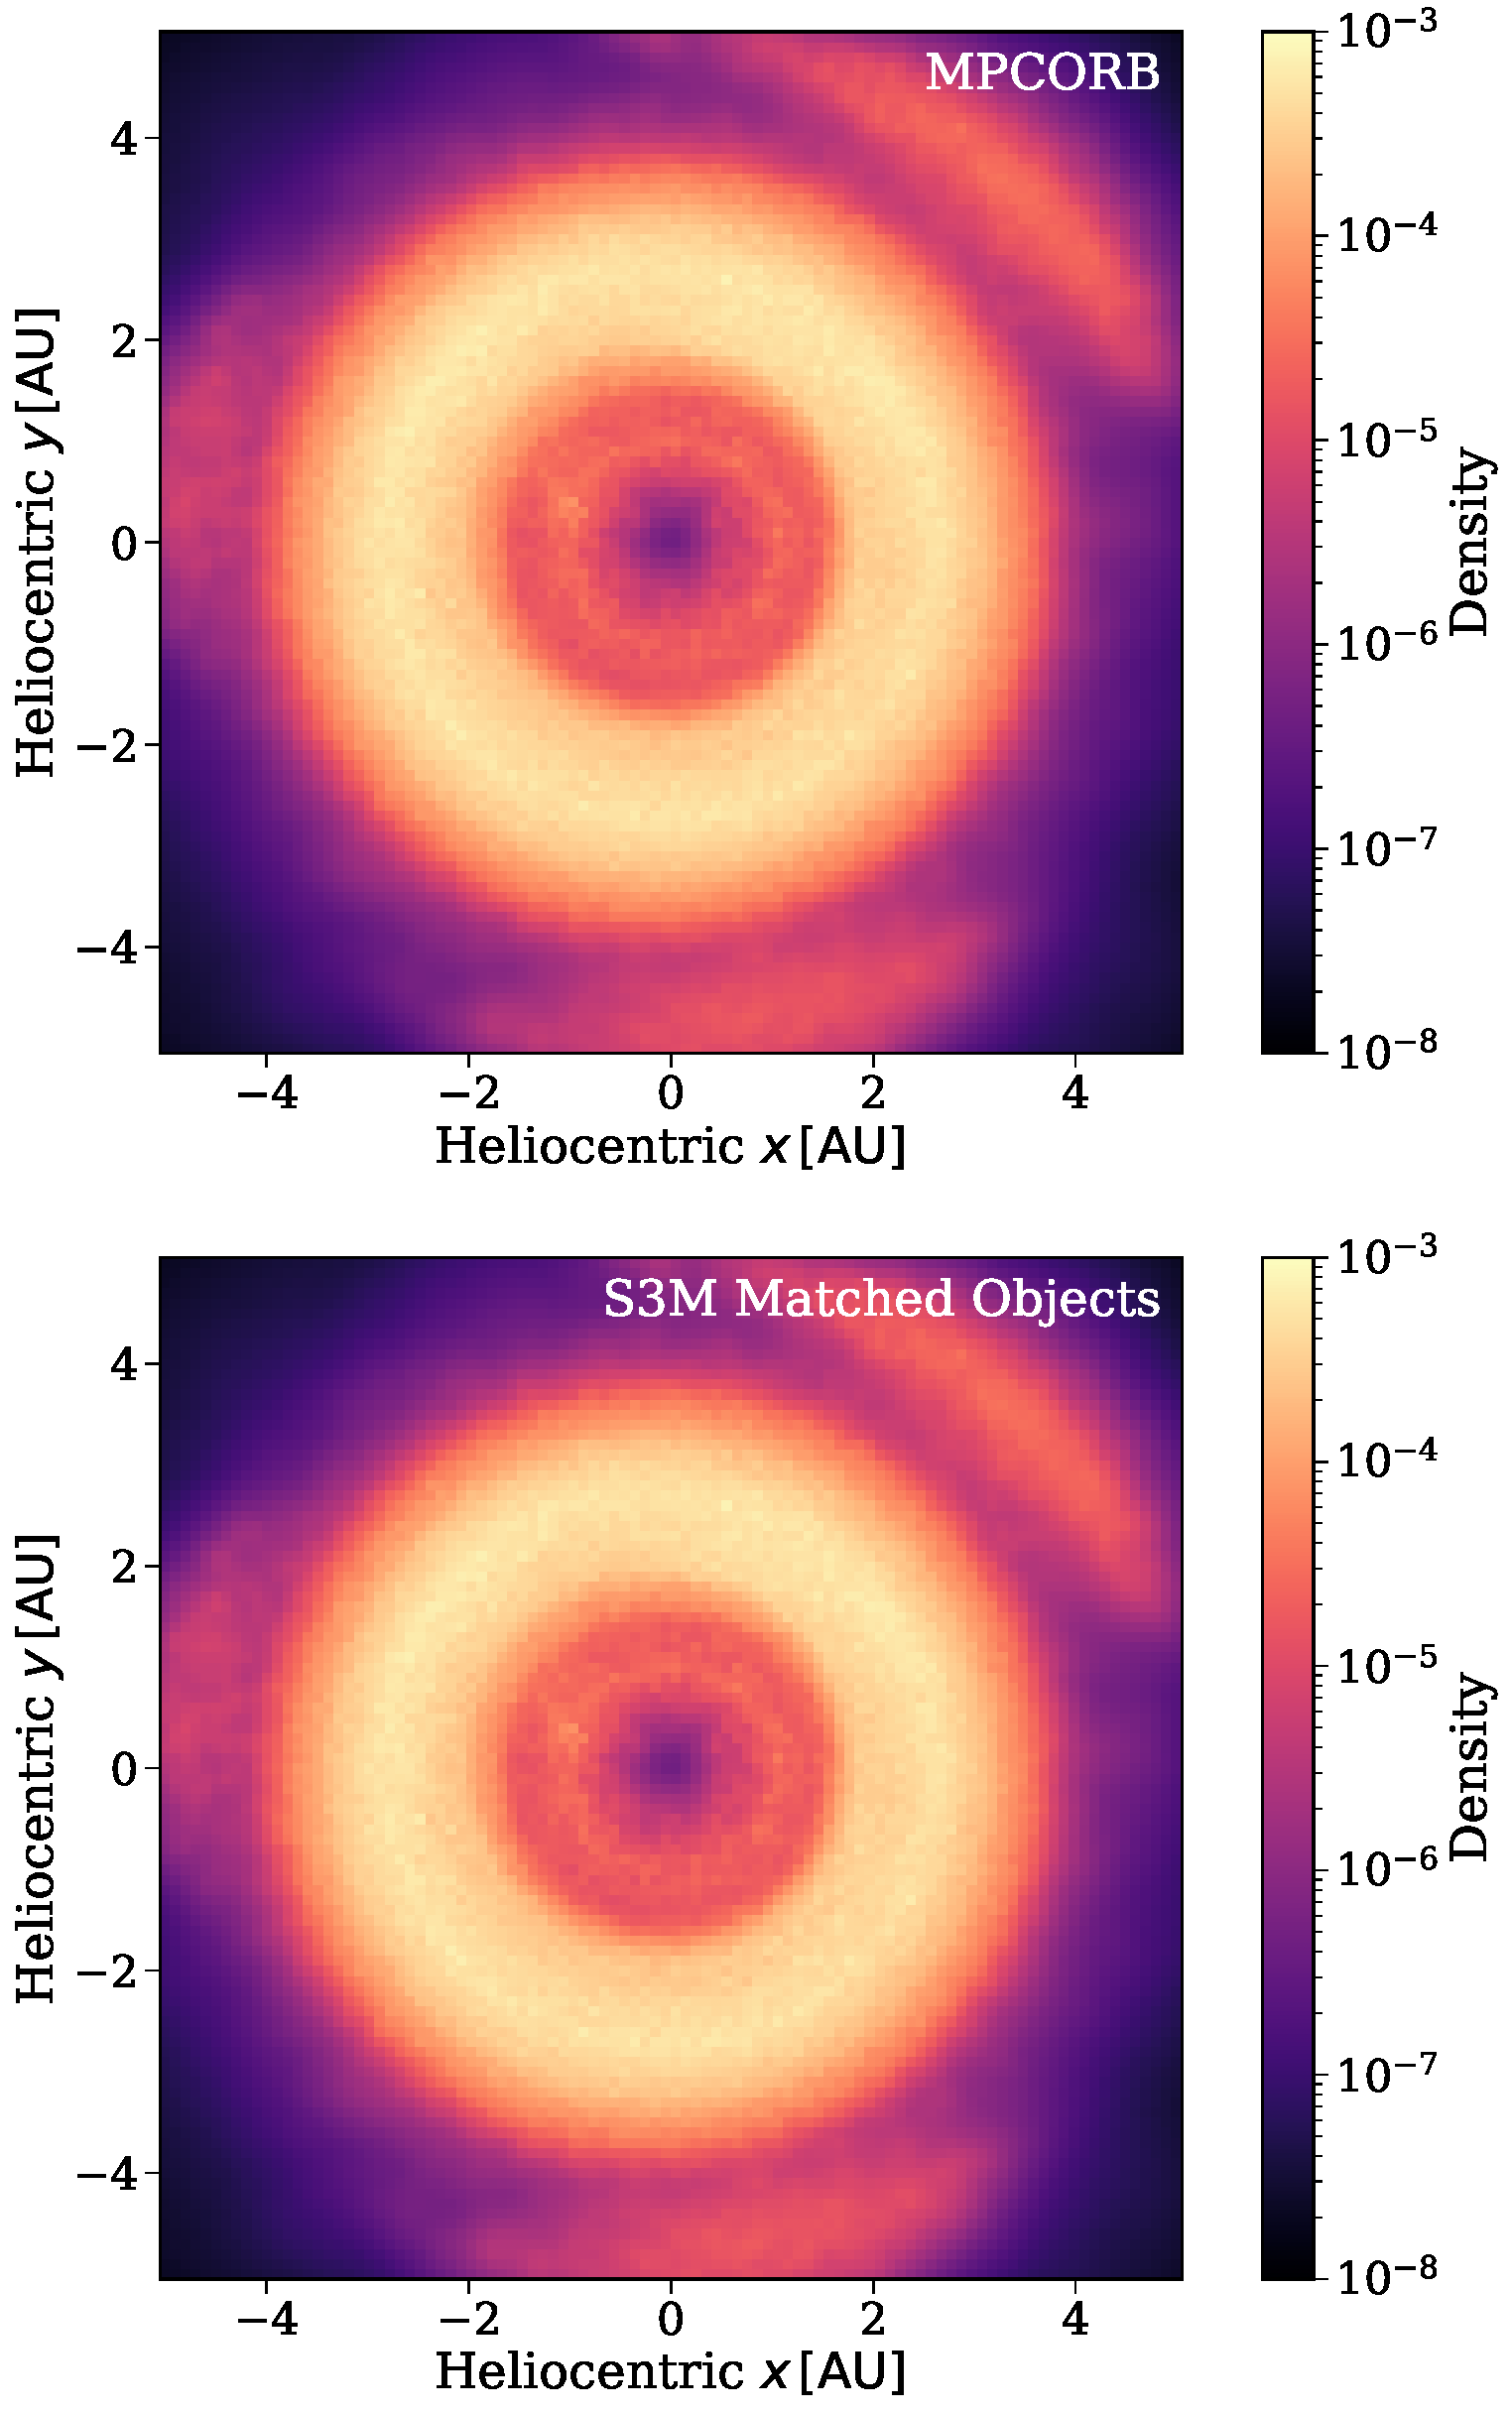
\includegraphics[width=0.48\textwidth]{density_comparisons.pdf}
    \raisebox{0.5\height}{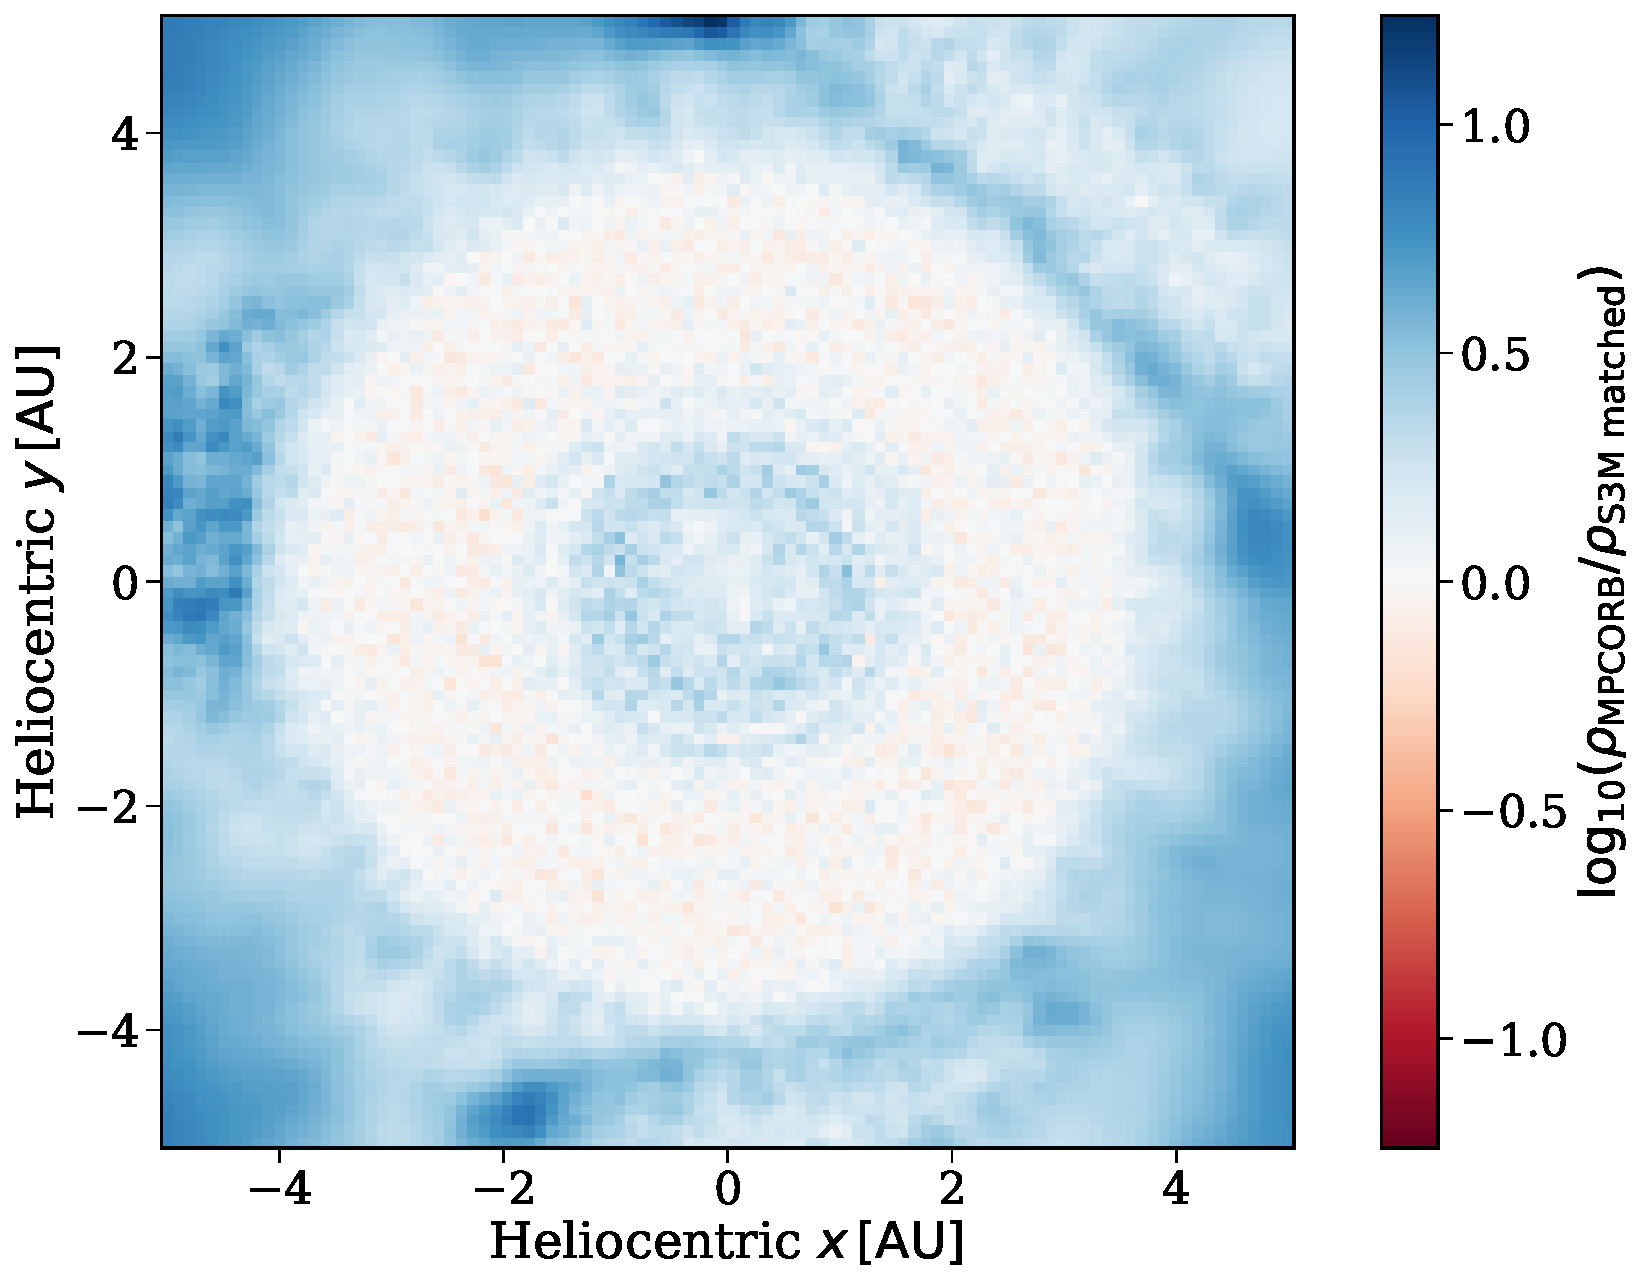
\includegraphics[width=0.48\textwidth]{density_residuals.pdf}}
    \caption{\textbf{Left:} A comparison of the density of \mpco{} objects with those objects that were matched in \sss{} by our hybrid catalogue pipeline. \textbf{Right:} Residuals between the two plots in the left panel.}
    \label{fig:density_compare}
\end{figure}

\end{document}